\documentclass[12pt,oneside,a4paper,bibtotoc,liststotoc]{scrreprt}
\usepackage{remreset}

%% Listings
\usepackage{listings}
\lstset{
  basicstyle=\footnotesize, 
  stringstyle=\ttfamily,
  frame=single,
  numberbychapter=false, % Listings vom Anfang bis zum Ende
                         % durchnummerieren
  captionpos=b
}
% Fußnoten, Tabellen und Grafiken von Anfang bis Ende durchnummerieren.
\usepackage{chngcntr}
\counterwithout{footnote}{chapter}
\counterwithout{table}{chapter}
\counterwithout{figure}{chapter}

% Überschriften bis zur dritten Ebene durchnummerieren
\setcounter{secnumdepth}{3}
% Überschriften bis zur zweiten Ebene in den TOC
\setcounter{tocdepth}{2}

%% Typographie-Schnickschnack
\usepackage[T1]{fontenc}
\usepackage{lmodern}
\usepackage{ellipsis} 

%% Absatzformatierung
% \parindent=0cm
\parskip=3mm

% Schönere Zeilenumbrüche
\usepackage{microtype}
\tolerance 1414
\hbadness 1414
\emergencystretch 1.5em
\hfuzz 0.3pt
\vfuzz \hfuzz
\raggedbottom
% Schusterjungen und Hurenkinder unterdrücken
\clubpenalty = 10000 
\widowpenalty = 10000 
\displaywidowpenalty = 10000 
% Schuster- und Hurenfußnoten will auch keiner...
\interfootnotelinepenalty=10000 

\usepackage[utf8]{inputenc}
% Mathematischen Formelsatz erlauben
\usepackage{amsmath}
\usepackage{amssymb}
\usepackage[ngerman]{babel}

%% Wenn ein Index verwendet werden soll, folgendes auskommentieren
% \usepackage{makeidx}
% \makeindex

\usepackage{graphicx}

% Erlaube das Setzen von anderne Zeilenabständen (s.u.)
\usepackage{setspace} 

%% Literaturverzeichnis
%\bibliography{MasterThesis_Konzepte_der_Nebenläufigkeit_v1.0}
\usepackage[round]{natbib}
\bibliographystyle{plainN}
%\bibliographystyle{IEEEtranN}
%\bibliographystyle{unsrt}
%\usepackage{jurabib}
%\jurabibsetup{
%	authorformat=abbrv,
%        titleformat={short,commasep},
%	commabeforerest,
%	see,
%        super, %% Konvertiert alle \cite in \footcite
%        square,
%        citefull=first,
%}
% Typographischer Schnickschnack für Bibliographie
%\renewcommand*{\jbauthorfont}{\textsc}
%\renewcommand*{\biblnfont}{\scshape\textbf}
%\renewcommand*{\bibfnfont}{\normalfont\textbf}

%% % Abstand vor Kapitelüberschriften: 0 cm (um es Bündig zu setzen, negativen Skip verwenden)
\renewcommand*{\chapterheadstartvskip}{\vspace*{0cm}}
%% % Abstand nach Kapitelüberschriften: 1 Zeile
\renewcommand*{\chapterheadendvskip}{\vspace{1\baselineskip}}

% Referenzen verlinken
\usepackage{hyperref}
\hypersetup{ 
    colorlinks,
    citecolor=black,
    filecolor=black,
    linkcolor=black,
    urlcolor=black 
}

% Grad-Zeichen definieren
\newcommand{\grad}{\mbox{\(\mathsurround=0pt{}^\circ\)}}
% (r)-Zeichen definieren
\def\TReg{\textsuperscript{\textregistered}}
% z.B., d.h. usw. Typographisch korrekt setzen
\usepackage{xspace}
\newcommand{\zB}{\mbox{z.\,B.}\xspace}
\newcommand{\dH}{\mbox{d.\,h.}\xspace}
\newcommand{\ua}{\mbox{u.\,a.}\xspace}
\newcommand{\so}{\mbox{s.\,o.}\xspace}
\newcommand{\MSc}{\mbox{M.\,Sc.}\xspace}
\newcommand{\BSc}{\mbox{B.\,Sc.}\xspace}


%% Schönere Tabellen
\usepackage{booktabs}
\usepackage{tabularx}

%% Ränder setzen
\usepackage[left=5cm,right=3cm,top=1.5cm,bottom=2cm,includeheadfoot]{geometry}

%% Abkürzungsverzeichnis
\usepackage[printonlyused]{acronym}

%% Allow really fixed positions for Tables
\usepackage{float}
\restylefloat{table}

%% Gedrehte Tabellen
\usepackage{rotating}

%% Trennung tweaken: Manche Wörter will man ggf. anders trennen als
%% der Algorithmus das vorsieht oder ggf. auch garnicht
\hyphenation{Java-Script}
\hyphenation{Cookies}

\begin{document}
\begin{titlepage} 
\begin{figure}[H]
  \begin{flushright}
    
\includegraphics{img/fh-koeln-logo.png}
    \label{logo_fh_köln}
  \end{flushright}
\end{figure}

\begin{center}
\textbf{\Large\newline  Fachhochschule Köln\\
Cologne University of Applied Sciences\\[0.1cm]
\normalsize Campus Gummersbach\\
Fakultät für Informatik und Ingenieurwissenschaften\\[0.5cm]}

 
\Large Verbundstudiengang Wirtschaftsinformatik\\[0.5cm]

\large Masterthesis\\[0.1cm]
  
% Title
{ \huge \bfseries \ Konzepte der Nebenläufigkeit  \\[0.1cm]
        unter Android \\[0.5cm]
        
}
\vfill

\begin{table}[h]
\centering
\begin{tabular}{ll}
  Prüfer:         & Prof. Dr. Erich Ehses \\
  Zeitprüfer:     & Prof. Dr. Frank Victor \\
  vorgelegt am:   & \today \\
  von cand.:      & Stephan Wagner \\
  aus:            & Overath \\
  Telefon-Nr.:    & +49-176-80007570 \\
  Matrikel-Nr.:   & 1106011828 \\
  E-Mail-Adresse: & stephan.wagner.mi738@gmail.com
\end{tabular}
\end{table}
\end{center}
\end{titlepage}



\onehalfspacing % 1,5-facher Zeilenabstand

\chapter*{Zusammenfassung}
Diese Thesis behandelt das Thema „Konzepte der Nebenläufigkeit unter Android“. Darin wird zunächst als Einführung in die Thematik, die Nebenläufigkeit allgemein mit ihren unterschiedlichen Ausprägungen (Prozess-/Threadebene) erläutert und die Risiken die mit Nebenläufigkeit einhergeht skizziert. Dabei ist ein besonders wichtiger Punkt der Botschaftenaustausch, der mittels unterschiedlicher Techniken realisierbar ist. Auch hier birgt jede Technologie ihre individuellen Vor- und Nachteile.
Die Nebenläufigkeit unter Android unterliegt einigen Besonderheiten, die sich teilweise aus den Restriktionen des Betriebssystems ergeben, aber auch aus den Anforderungen für die Android Applikationsentwicklung, die der StyleGuide vorgibt. So ist die grundsätzliche Anforderung, dass Applikationen ansprechbar bleiben. Eine Applikation, insbesondere eine Gui Applikation sollte somit beim Start von Operationen weder blockieren oder nicht mehr auf Benutzereingaben reagieren. Technisch bedeutet dies, dass zeitaufwändige Operationen nie auf dem Main Thread der Applikation stattfinden dürfen. Stattdessen müssen derartige Operationen in Hintergrundthreads ausgelagert werden. Im Kapitel 2 werden hierzu drei unterschiedliche Konzepte an Hand konkreten Beispielimplementierungen vorgestellt und in der jeweiligen Funktionsweise analysiert.
\begin{itemize}
\item Java Concurrency nach Java SE
\item Android Concurrency aus dem Android SDK
\item RXJava Framework
\end{itemize}
Die aus der technischen Analyse gewonnenen Erkenntnisse werden in Kapitel 3 genutzt um Chancen und Risiken der einzelnen Konzepte zu diskutieren. Um die Ergebnisse aus dem Diskurs für zukünftige Entscheidungsfindungen zu Rate ziehen zu können fließen die aus der Detailanalyse gewonnenen Ergebnisse in eine Szenarien basierte Analyse ein, um daraus Anhaltspunkte für den sinnvollen Einsatz der Konzepte abzuleiten.

\tableofcontents
\listoffigures


\chapter{Einleitung}
\section{Motivation}
Mobile Endgeräte begleiten immer mehr Menschen in ihrem Alltag. Damit einher geht die intensive Nutzung von sog. Apps., womit Applikationen auf den mobilen Endgeräten bezeichnet werden. Mit der zunehmenden Leistungsfähigkeit der Geräte werden auch immer komplexere Applikationen realisierbar. Wurde zu den Anfängen der Applikationsentwicklung für mobile Endgeräte lediglich einfache Funktionalität in Applikationen integriert, werden heute mit unter teilweise sehr rechenintensive und komplexe Funktionalitäten entwickelt. Eine optimale Konzeption der Aufgabenverarbeitung innerhalb der Applikation kann dabei einen entscheidenden Faktor für die Performance und damit auch die Akzeptanz beim Nutzer darstellen. Damit gewinnt die Nebenläufigkeit auch in der Applikationsentwicklung für mobile Endgeräte an Wichtigkeit. Nebenläufigkeit oder auch Parallelverarbeitung bezeichnet in der Informatik die Eigenschaft eines Programms oder eines Systems verschiedene Aufgaben zeitgleich, also parallel zu bearbeiten. Die jeweilige Verarbeitung kann dabei in sich abgeschlossen sein, d.h. die zu verarbeitenden Aufgaben sind voneinander unabhängig, oder die Verarbeitung hängt von den Ergebnissen aus anderen Aufgaben ab. Je nach Art und Weise der Parallelverarbeitung sind verschiedene Problematiken und Risiken zu beachten. Für Nebenläufigkeit unter dem Android Betriebssystem sind zusätzliche Besonderheiten zu beachten. Dieses Betriebssystem ist auf mobile Endgeräte zugeschnitten und hat diesbezüglich spezielle Anforderungen an Applikationen die darauf laufen sollen. Die Firma Google als Hersteller vom Betriebssystem Android legt hierbei großen Wert auf die Einhaltung eines StyleGuides der die Benutzbarkeit applikationsübergreifend in einem einheitlichen Standard definiert. Darin wird die grundlegende Anforderung nach der kontinuierlichen Ansprechbarkeit von Applikationen gefordert. Die Frage ist wie kann den Anforderungen an Android Applikationen mittels unterschiedlicher Konzepte der Nebenläufigkeit begegnet werden, sodass das von Google geforderte Ziel der Ansprechbarkeit erreicht werden kann. Welche Problemstellungen, Restriktionen oder Risiken gehen mit der Verwendung bestimmter Konzepte einher und wie praktikabel sind diese für den konkreten Praxiseinsatz? 

\section{Zielsetzung und Vorgehen}
In dieser Arbeit soll untersucht werden, wie konkurrierende Parallelverarbeitung in mobilen Anwendungen realisiert werden kann. Dabei besteht das Ziel, die Entwicklung von Nebenläufigkeit durch Verwendung unterschiedlicher Techniken zu vereinfachen und ggf. auf einem höheren Abstraktionsniveau ab zu bilden. Zunächst gilt es in einer kurzen Einführung in die Thematik, die grundsätzlichen Definitionen kurz zu erläutern und auf Besonderheiten der Parallelverarbeitung unter Android einzugehen. Weiter wird ein Überblick über eine Auswahl von unterschiedlichen Konzepten der Nebenläufigkeit unter Android erarbeitet. Diese werden mittels einfacher Beispiele vorgestellt und analysiert. Den Abschluss bildet ein kritischer Diskurs, um in Abhängigkeit vom Einsatzkontext eine Differenzierte Sicht auf die Anwendung der einzelnen Konzepte zu erhalten. Die Ergebnisse des Diskurses werden in einer szenarienbasierten Analyse aufgegriffen um diese greifbarer zu machen.

\section{Begriffsdefinition und Grundlagen der Nebenläufigkeit}
Um sich den Konzepten der Nebenläufigkeit anzunähern, werden zunächst einige Begriffsdefinitionen benötigt. Die Nebenläufigkeit meint dabei konkret die parallele Verarbeitung von Aufgaben. Hierzu wird eine Aufgabe in Unteraufgaben aufgeteilt, um diese  weitestgehend von einander unabhängig abzuarbeiten. Die Definition wie diese Verarbeitung ablaufen soll, ist in einem Programm hinterlegt. Die Ausführung von Programmen wird von Prozessen und Threads geregelt. Diese werden im folgenden Abschnitt definiert und ein tieferes Verständnis von der Parallelverarbeitung auf Betriebssystemebene erarbeitet.

\section{Prozesse und Threads}
Die genauen Eigenschaften von Prozessen und Threads sind abhängig vom Betriebssystem auf dem sie laufen. Da in dieser Arbeit der Fokus auf Nebenläufigkeit unter Android liegt, beziehen sich die folgenden Erläuterungen zu Prozessen und Threads auf das allgemeine Unix/Linux Betriebssystem auf dem Android basiert.

\subsection{Prozess}
Wird eine Anwendung gestartet, so erzeugt das Betriebssystem zunächst einen Prozess, der den Adressraum für sämtliche Programmdaten und Komponenten reserviert. Für Prozesse kann folgende Definition getroffen werden. Sie gilt betriebssystemübergreifend:
\begin{center}
Ein Prozess stellt ein Programm in Ausführung dar und
ist für die Kontrolle(Sicherung) der damit verbundenen Betriebsmittel
verantwortlich.
\end{center}
Die Prozesse sind (in der Regel) an einen Benutzer gebunden, welcher wiederum über bestimme Rechte u.a. im Dateisystem verfügt. Dabei sind für Linux Betriebssysteme folgende Prinzipien zu beachten:
\begin{itemize}
\item Hierarschische Prinzip
\item Sandbox Prinzip
\end{itemize}
Das hierarchische Prinzip schreibt die Abhängigkeit von Prozessen gegenüber ihren Erzeugern vor. Mit Ausnahme des Root Prozesses des Betriebssystems, werden alle Anwendungen durch einen Vater Prozess erzeugt. Die damit verbundene Vater-Kind Abhängigkeit bildet eine Baumstruktur, in der jeder Prozess seinen erzeugenden Prozess kennt. Ein Prozess kann nur aus anderen Prozessen heraus erzeugt werden. Stirbt ein Prozess, so werden die Kind Prozesse in der Regel vom Root Prozess des Betriebsystems adoptiert.\newline
Das Sandbox Prinzip ist ein Sicherheitskonzept aus dem Kern eines Linux/Unix Betriebssystems. Darin wird sichergestellt, dass jede Anwendung nur die eigenen Daten sehen darf. So wird bei der Installation für jede Anwendung ein eigener Betriebssystem- User erzeugt, der über spezielle Rechte zu Prozessen und Dateien verfügt. Damit wird zum Ausführungszeitpunkt verhindert, dass Programmdaten für andere Programme sichtbar werden. Die Sicht jedes Prozesses einer Anwendung ist begrenzt auf die Ressourcen die dem jeweiligen Betriebssystem User zugeordnet sind.

\subsection{Thread}
Die Begriffe Prozesse und Threads dürfen nicht synonym verwendet werden. So kann ein Thread wie folgend Definiert werden:
\begin{center}
Ein Thread stellt einen Ausführungsfaden
eines Programmes dar.
\end{center}
Dieser besteht aus aus einem aktuellen Befehlszeiger, einem eigenen Stack und dem Inhalt der Prozessorregister. Zum Start einer Anwendung wird der sog. Main Thread erzeugt. Aus diesem lassen sich beliebig weitere Threads erzeugen. Dabei besteht keine hierarchische Bindung wie bei der Vater-Sohn Prozesshierarchie. Innerhalb eines Prozesses erzeugte Threads erhalten Zugriff auf den hier reservierten Speicher des Prozesses. Alle in einem Prozess erzeugte Threads sind von diesem abhängig. Wird demnach ein Prozess terminiert, so werden auch alle darin erzeugte Threads terminiert.

\section{Botschaftenaustausch und Kommunikation}
Der Botschaftenaustausch zwischen Prozessen unterscheidet sich vom Botschaftenaustausch zwischen Threads. Während bei der Inter Prozess Kommunikation maßgeblich das Betriebssystem am Austausch von Nachrichten zwischen Prozessen beteiligt ist, können bei der Inter Thread Kommunikation unterschiedliche Techniken unabhängig vom Betriebssystem angewandt werden. Für die Kommunikation zwischen Threads eignen sich z.B. Dateien aber auch sogenannte MessageQueues mit denen Produzenten und Konsumenten Konstrukte erzeugt werden können. Die Inter Thread Kommunikation bleibt begrenzt auf die Threads innerhalb einer Anwendung. Die Inter Prozess Kommunikation dagegen, definiert die Kommunikation über Programm- und Systemgrenzen hinaus. Innerhalb eines Betriebssystems wird in der Regel der Speicherbereich jedes Prozesses in sich gekapselt und vor anderen Prozessen verborgen (s.o. Sandbox-Prinzip). Daher werden Mechanismen seitens des Betriebssystems benötigt (Botschaftenaustausch über Socket, etc..) um die Kommunikation zu gewährleisten. Diese Mechanismen sind aufwendig und eignen sich dadurch weniger für eine effiziente Parallelverarbeitung. Daher konzentriert sich diese Arbeit auf die Kommunikation auf Thread Ebene, und die Inter- Prozess Kommunikation wird nicht weiter thematisiert. Die folgenden Abschnitte geben einen Einblick auf gängige Techniken zur Realisierung von Inter- Thread Kommunikation.

\subsection{Geteilte Datei/ Speicher}
Einer der einfachsten technischen Mittel für den Daten- /Botschaftenaustauch ist die Nutzung einer gemeinsamen Datei im Dateisystem des Betriebssystems. Dadurch, dass das Betriebssystem den exklusiven Zugriff auf Dateien gewährleisten kann, ist es möglich ohne großen Aufwand eine synchronisierte Kommunikation zu realisieren. Etwas komplexer ist es für die Kommunikation einen Speicherbereich zu allokieren und die Referenz darauf den jeweiligen Kommunikationspartern für den Datenaustausch zur Verfügung zu stellen. In diesem Fall muss der exklusive Ausschluss selbst realisiert werden, falls er gewünscht ist. Hierzu dienen einfache Primitive aus dem java.lang.concurrency Packet.

\subsection{MessageQueues}
Die folgende Abbildung gibt einen schematischen Überblick über die Nutzung einer MessageQueue für die Kommunikation zwischen Objektinstanzen aus unterschiedlichen Threads. Beide Objekt Instanzen müssen eine Referenz auf das MessageQueue Objekt halten um Nachrichten (z.B. Message to Thread B) in diese Queue einzustellen oder herauszuholen. Das Konzept des nachrichtengetriebenen Datenaustausches hat den Vorteil, dass jede Nachricht eine atomare (in sich geschlossene) Einheit darstellt. Dadurch lassen sich einzelne Arbeitsaufträge unterscheiden. Je nach Implementierung der MessageQueue sind auch keine weiteren Synchronisationen mehr nötig.
\begin{figure}[H]
  \begin{centering}
    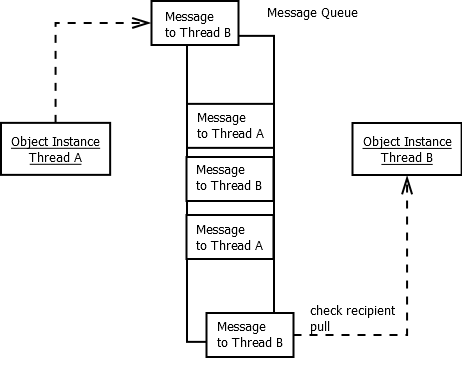
\includegraphics[width=0.8\textwidth]{img/MessageQueue.png}
    \caption{MessageQueue}
    \label{MessageQueue}
  \end{centering}
\end{figure}
Die Kommunikation mittels einer MessageQueue kann in zwei Formen realisiert werden:
\begin{itemize}
\item Unidirektional
\item Bidirektional
\end{itemize}
Bei der unidirektionalen Kommunikationsform darf ein Kommunikationspartner nur entweder Nachrichten aus der Queue entnehmen oder hinein geben. In unserem Beispiel dürfte demnach nur die Objekt Instanz des Thread A Nachrichten in die Queue geben und die Objekt Instanz des Thread B darf lediglich aus dieser lesen.\newline
Bei der bidirektionalen Kommunikationsform dürfen beide Kommunikationspartner je Nachrichten in die MessageQueue einstellen wie auch herausnehmen.\newline 
\newline

Die letzten beiden Abschnitte haben einen Überblick über Technologieen gegeben, mit denen der Austausch von Informationen innerhalb einer nebenläufigen Verarbeitung über Thread Grenzen hinaus realisiert werden kann. Dabei stellen MessageQueues eine Abstraktionsebene zur Kommunikation über fest definierten Speicher dar. Die Entwicklung von Nebenläufigkeit kann jedoch auch zu schwerwiegenden Problemen führen.


\section{Risiken von Nebenläufigkeit}
Der Botschaftenaustausch zwischen Threads, sowie deren Synchronisation kann zu schwerwiegenden Problemen im Zuge der Prallelverarbeitung führen. Folgende Szenarien sind eher allgemein gehalten, jedoch gilt es, besonders in dem Kapitel 2  zu den konkreten Implementierungen von Nebenläufigkeit, diese Problematiken zu beachten. In Kapitel 3 werden die in Kapitel 2 zu diskutierenden Beispielimplementierungen u.a. an Hand der hier aufgeführten Risikoszenarien und dem damit verbundenen Fehlerpotential bewertet.

\subsection{Philosophenproblem}
Ein zentrales Problem der theoretischen Informatik ist das Philosophenproblem das erstmals beschrieben wurde durch Edsger W. Dijkstra. Darin wird ein Szenario berschrieben, in dem eine bestimmte Anzahl von Philosophen auf begrenzte Ressourcen zugreifen und bei gleichzeitigem Zugriff sich gegenseitig blockieren können.

\begin{figure}[H]
  \begin{centering}
    
\includegraphics[width=0.6\textwidth]{img/PhilosophenProblem.png}
    \caption{Philosophenproblem \cite[]{philosofen}}
    \label{Philosophenproblem}
  \end{centering}
\end{figure}
Die Abbildung zeigt wie eine Gruppe von Philosophen an einem Runden Tisch sitzen, vor ihnen etwas zu Essen. Um zu essen, benötigen nach diesem theoretischen Aufbau die Philosophen die rechte und die linke Gabel neben dem jeweiligen Teller. Dabei versuchen die Philosophen zu nächst die Gabel zu ihrer Linken zu nehmen. Ist die Gabel frei, so behalten sie diese in der Hand bis auch die Gabel auf der rechten aufgenommen werden kann. Kann ein Philosoph eine Gabel zur Zeit nicht nehmen, da sie in Verwendung ist, verweilt er denkend bis die benötigte Gabel frei ist. Versuchen jedoch alle Philosophen gleichzeitig die Gabeln aufzunehmen, so besteht die Gefahr einer Verklemmung (engl. Deadlock). Der Ablauf stockt und die Philosophen verharren denkend bis sie verhungern. In Bezug auf die Kommunikation über geteilten Speicher oder Dateien kann dieses Problem auftreten wenn parallele Zugriffe auf exklusive Ressourcen nicht sauber synchronisiert werden.



\subsection{Race Conditions}
Ein weiteres Problem bei der Parallelverarbeitung tritt bei geteilten Speicher bzw. Daten auf. Folgende Abbildung illustriert das Szenario, dass drei Threads auf einen gemeinsamen Speicherbereich zugreifen. Die Threads eins bis drei greifen konkurrierend lesend, wie schreibend auf den Speicherbereich zu und tauschen darüber Informationen untereinander aus. Der Zugriff erfolgt nach dem Prinzip \glqq Wer zuerst kommt mahlt zuerst\grqq  ( = Race Condition).

\begin{figure}[H]
  \begin{centering}
    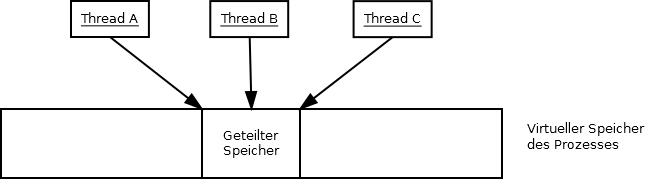
\includegraphics[width=0.8\textwidth]{img/SharedMemory_RaceCondition.png}
    \caption{Geteilter Speicher bei der Inter-Thread Kommunikation}
    \label{SharedMemory_RaceCondition}
  \end{centering}
\end{figure}
Ist der Zugriff der Threads auf den Speicher nicht synchronisiert, so kommt es zu dem Shared Memory Effekt, (geteilter Speicher Effekt) nach dem eine Datenstruktur die, die Grundlage von Berechnungen darstellt, durch einen anderen Thread verändert wird, ohne dass die Änderung dem ersten Thread bekannt gemacht wird. Da solche Probleme von der jeweils in diesem Moment vorliegenden Prozessauslastung im System abhängen (tatsächlich gleichzeitig laufende Threads im Multi Core System), sind derartige Effekte schwer reproduzierbar und somit auch die Ursachen schwer zu finden.


\subsection{Speicherleck}
Speicherlecks (eng. Memory Leaks) entstehen häufig aus Programmierfehler heraus, in denen Speicher reserviert, aber dieser nicht mehr freigegeben wird. Geschieht dies ausreichend oft während einer Laufzeit innerhalb des Addressraums des Programmes, so gerät im schlimmsten Fall der seitens der Hardware begrenzte Speicher an seine Grenzen. Das Betriebssystem registriert dieses Verhalten und terminiert sofort die Ausführung des Programmes. Bei der Technik des geteilten Speichers, ist das Risiko eines Speicherlecks z.B. dann präsent, wenn sich der Entwickler um korrekte Dereferenzierung des Speichers und dessen Freigabe explizit kümmern muss. Wird Speicher n-Fach allokiert und nicht wieder freigegeben, so handelt es sich um ein ernstes Speicherleck. Auch bei der MessageQueue sind Speicherlecks möglich, z.B. wenn kontinuierlich Botschaften in die Queue gepackt werden, diese aber nicht aus der Queue wieder herausgenommen werden.

\subsection{Reihenfolgeproblem}
Im Falle einer bidirektionalen Kommunikation mittels einer MessageQueue muss beachtet werden, dass es nicht vorhersehbar ist, in welcher Reihenfolge die Nachrichten in die MessageQueue gelegt werden, oder wann sich welcher Thread eine Message aus der Queue holt. Dies kann zu unerwarteten Verhalten führen. So kann ein Thread B ungewollt blockieren, wenn er für seine weitere Verarbeitung eine bestimmte Nachricht benötigt und diese jedoch sich in der Reihenfolge hinter einer Nachricht für den anderen Thread A befindet. So muss Thread B solange warten bis Thread A seine Nachricht aus der Queue nimmt.
\newline
Welche Konzepte es gibt, um sich den allgemeinen Problematiken und Risiken von Nebenläufigkeit speziell für Android Applikationen zu nähern ist zentraler Forschungsschwerpunkt dieser Arbeit. Diese Konzepte werden im Kapitel 2 im einzelnen vorgestellt.


\section{Parallelverarbeitung und Besonderheiten unter Android}
Im vorangegangenen Abschnitt wurde allgemein auf die Terminologie, die Eigenschaften, sowie die Kommunikation innerhalb von Nebenläufigkeit eingegangen. Hier gilt es nun einen Fokus auf Nebenläufigkeit im mobilen Umfeld zu setzen, insbesondere unter dem Betriebsystem Android. Weiter wird ein erster Einblick in das Komponentenmodell, sowie in den Lebenszyklus von Android Applikationen erarbeitet.


\subsection{Prozesse und Threads unter Android}
\paragraph{Prozess Charakteristika}
Das Android Betriebssystem basiert auf dem Linux/Unix System. Daher gelten die o.g. Eigenschaften zu Prozessen unter dem Linux/Unix Betriebssystem auch für Android. Sie werden lediglich um folgende Charakteristika erweitert.
\begin{enumerate}
\item Fordergrundprozess $\rightarrow$ Fordergrundprozesse sind verantwortlich für alle Komponenten einer Anwendung, die unmittelbar im Vordergrund, also für den Nutzer sichtbar sind.
\item sichtbarer Prozess $\rightarrow$ Sichtbare Prozesse fassen alle Komponenten zusammen, die zwar nicht unmittelbar sichtbar sein müssen, jedoch Komponenten aus dem Vordergrund beeinflussen.
\item Service Prozess $\rightarrow$  Service Prozesse laufen losgelöst von anderen Prozessen. Einmal gestartet laufen diese selbstständig (z.B. das Abspielen von Musik). Sie lassen sich jedoch weiterhin von anderen Prozessen steuern.
\item Hindergrundprozess $\rightarrow$ Der Hintergrundprozess hält gestoppte Anwendungskomponenten. So werden darin Activity Instanzen abgelegt, für welche die onStop() Methode (siehe Activity Lifecyle) aufgerufen wurde. Dies hat die Funktion, die Anwendung möglichst schnell wieder zu reaktivieren, wenn der Nutzer dies wünscht. Der Hintergrundprozess darf nicht mit der im folgenden Kapitel thematisierten Hintergrundverarbeitung zusammen in einen Kontext gebracht werden.
\item leerer Prozess $\rightarrow$ Leere Prozesse werden bei ausreichend Hardware Ressourcen durch das Android Betriebssystem erzeugt und als Ressourcen für einen schnelleren Start von Applikationen gehalten. Wünscht ein Nutzer eine Anwendung zu starten, so existiert bereits hierfür ein Prozess mit entsprechender Laufzeitumgebung.
\end{enumerate}
Rein aus der Sicht des Betriebsystems handelt es sich stets um den gleichen Prozess, jedoch kann er unterschiedliche Charakteristika innerhalb seines Lebenszyklus annehmen.
\paragraph{Sandbox Prinzip}
Eine weitere Besonderheit in Android erweitert das Sandbox Prinzip von Unix/Linux Systemen zur Kapselung von Prozessen und deren Ressourcen (siehe Abschnitt 1.2.1 “Prozesse und Threads”). Dabei erzeugt Android bereits zum Installationszeitpunkt pro Anwendung einen speziellen User. Wird die Anwendung gestartet, so richtet das Betriebssystem einen in sich geschlossenen Speicherbereich ein und ordnet diesen dem jeweiligen Appliction-User zu. Somit wird der exklusive Zugriff auf den Speicherbereich allein durch diese Applikation realisiert.

\paragraph{UI-Thread als Main Thread}
Bei der Entwicklung von Android Applikationen steht die Benutzerschnittstelle im Vordergrund. So erscheint es konsequent, dass das User Interface durch den Main Thread verarbeitet wird (hier gilt also Main-Thread = UI-Thread). Dieses Ausführungsmodell steht z.B. dem von Java.Swing entgegen, in welchem die Benutzerinteraktion in einem sekundären Thread, ungleich dem Hauptthread gesteuert wird. Dies hat unweigerlich Einfluss auf die Konzeption von Applikationen unter Android,
 welche u.a. zeitintensive Operationen durchführen müssen. Denn in diesem Fall darf der UI Thread nicht blockieren und sich nach Ende der Verarbeitung erst wieder zurück melden. Die zeitintensive Operation muss in einen sekundär Thread ausgelagert werden, sodass der UI Thread weiter Benutzereingaben verarbeiten kann.

\subsection{Besonderheiten im Android Umfeld bezüglich des Thread Managements}
Das Android Betriebssystem formuliert einige spezielle Regeln für die Ausführung von Threads, die sich an einen hohen Anspruch seitens Google an der Benutzbarkeit der Applikationen orientieren. So ist der Thread für die Steuerung der Benutzeroberfläche (User Interface kurz UI) unter besonderer Beobachtung. Wird dieser Blockiert oder ist ausgelastet mit zeitintensiven Operationen, wird dieser vom Betriebssystem nach einer bestimmen Zeit angehalten. Je nach Konfiguration des Android Betriebssystems wird es dem Nutzer angeboten entweder weiter zu warten oder die Applikation zu terminieren.

\subsubsection{ANR Dialog}
Ein grundsätzlicher Anspruch, den Google an mobile Anwendungen unter seinem Android Betriebssystem stellt, ist die Benutzbarkeit durch den alltäglichen Anwender. Dieser muss über keine technischen Kenntnisse verfügen um die Applikation entsprechend einfach und intuitiv benutzen können. So ist es unerwünscht, dass eine Applikation nach dem Start irgend eines Vorganges blockiert, also auf Interaktion des Nutzers nicht reagiert. Google formuliert in seiner Andorid Developper Dokumentation daher die grundsätzliche Anforderung der kontinuierlichen Ansprechbarkeit von Appliationen bzw. der nie zu unterbrechenden Interaktionsfähigkeit zwischen Benutzer und Applikation. So ist es gemäß der Designvorgaben für Android Applikationen unerwünscht, das Applikationen blockieren. Um jedoch für den Fall einer blockierenden Anwendung gerüstet zu sein, bietet Android die Möglichkeit, mittels eines Applikation Not Responding Dialogs, kurz ANR Dialog die Verarbeitung innerhalb einer Anwendung abzubrechen oder weiter auf deren Ergebnis zu warten. Wird im Dialog auf \glqq Warten\grqq geklickt, gibt das Betriebssystem den UI Thread wieder zur Ausführung frei. Folgende Abblildung zeigt einen exemplarischen ANR Dialog:
\begin{figure}[H]
  \begin{centering}
    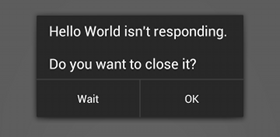
\includegraphics[width=0.6\textwidth]{img/anr-dialog.png}
    \caption{ANR Dialog unter Android}
    \label{ANR Dialog}
  \end{centering}
\end{figure}
In diesem Beispiel greift Android in den Lebenszyklus der Aktivity ein, von der die zeitintensive Berechnung ausgeht und pausiert diese. Je nach Wunsch des Nutzers wird die Applikaiton dann in den Status \glqq Pausiert\grqq überführt, oder terminiert (siehe: onStoped() bzw. onDestroyed() im Lifecycle Diagramm) und vom Garbage Collector entsorgt (siehe hierzu Lebenszyklus einer Activity im nächsten Abschnitt). Die Zeit T innerhalb derer eine Applikation nicht auf Benutzereingaben reagiert und deren Ablauf der genannte Dialog erscheint ist für jedes Android Gerät konfigurierbar. Obwohl diese Eingreifmöglichkeit eine wichtige Funktion für die Kontrolle von Applikation durch den Nutzer darstellt, haben sich diverse Gerätehersteller mittlerweile entschieden die Zeit T sehr groß zu wählen, oder sogar den ANR-Dialog generell zu deaktivieren. In den Android Versionen ab Honeycomb führt das Blockieren einer Applikation bereits zur sofortigen Terminierung durch das Betriebssystem. Doch unabhängig vom ANR-Dialog bleibt der direkte Zusammenhang zwischen der Ansprechbarkeit einer Applikation und der Benutzbarkeit der Anwendung und dem Nutzererlebnis. Blockiert über zu lange Zeit eine Anwendung, so steigt damit auch die Unzufriedenheit des Nutzers über die Anwendung, besonders da er häufig die technischen Zusammenhänge, welche eine zeitintensive Verarbeitung durch aus rechtfertigen können, nicht kennt und gemäß der angesprochenen Designvorgaben auch nicht kennen muss.


\subsubsection{Komponentenmodell}
Bisher wurde die technische Ausführung von Android Applikationen auf der Betriebssystemebene erläutert. Für die einzelnen Konzepte der Nebenläufigkeit unter Android gilt es nun jedoch näher auf die Konzeption von Applikationen mittels klar definierten Komponenten selbst ein zu gehen, bevor im Kapitel 2 die einzelnen Konzepte an konkreten Implementierungsbeispielen verdeutlicht werden. Die folgende Abbildung zeigt die Basiskomponenten aus denen Anwendungen unter dem Android Betriebssystem bestehen:
\begin{figure}[H]
  \begin{centering}
    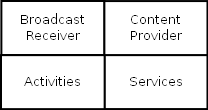
\includegraphics[width=0.6\textwidth]{img/Android_Komponent_Model.png}
    \caption{Komponentenmodell für Android Applikationen}
    \label{Android_Komponent_Model}
  \end{centering}
\end{figure}
\begin{itemize}
\item Broadcast Receiver erlauben die Registrierung von systemweiten oder applikationsinternen Events.
\item Content Provider repräsentieren Daten als relationalen Datensatz und ermöglichen den Zugriff über Applikationsgrenzen hinaus auf diese Daten.
\item Activities definieren das Verhalten von graphischen Benutzerschnittstellen
\item Services können zeitintensive Hintergrundberechnungen abbilden. 
\end{itemize}
Bei Services ist zu beachten, dass diese, wenn nicht anders definiert in dem Main Thread laufen, was jedoch für zeitintensive Verarbeitungen zu Problemen mit dem Benutzerinterface führen kann, wie in den folgenden Abschnitten näher beschrieben wird. Services dienen lediglich als mögliche Kapselung um Hintergrundverarbeitungen klarer vom Rest der Applikation zu trennen, sowie Verarbeitungen ohne aktives Benutzerinterface durchzuführen. Die Android Developper Dokumentation weist explizit darauf hin, keine zeitaufwändigen Verarbeitungen hier zu definieren wenn der Service im Main Thread läuft, da ansonsten die Gefahr besteht, dass der Main Thread und somit auch das Benutzerinterface blockiert. Dies gilt neben Services auch für die anderen Komponenten.

\subsubsection{Lebenszyklus einer Android Anwendung (Activity)}
Da sich diese Arbeit primär auf Applikationen mit Benutzerinterface konzentriert, macht es Sinn kurz auf den Lebenszyklus von Activities einzugehen der bereits in Kapitel \glqq Besonderheiten im Android Umfeld bezüglich des Thread Managements\grqq kurz aufgegriffen wurde.
Applikationen unter dem Android Betriebssystem unterscheiden sich in einigen Details deutlich von normalen Java Applikationen. Im Hinblick auf die nebenläufige Verarbeitung ist es daher von Bedeutung einen genaueren Blick auf den Lebenszyklus von Android Applikationen zu werfen. Die folgende Abbildung gibt einen Überblick über die Stati einer gestarteten Activity. Eine Objekt Instanz vom Typ android.os.Activity ist dabei der Einstiegspunkt in eine GUI-Applikation und wird vom Betriebssystem beim Start der Anwendung aufgerufen. Die einzelnen Statusübergänge, die in der Abbildung durch die jeweiligen Rückrufmethoden (onCreate(), onStart, onResume())symbolisiert werden,  sind für diese Arbeit weniger von Bedeutung. Interessanter sind die Abhängigkeiten zum Lebenszyklus des Prozesses, welcher für die Anwendung gestartet wurde, und damit die Frage nach der Lebensdauer von Threads. Die Abbildung zeigt deutlich zwei Szenarien in denen jeweils die Anwendung aus dem Sichtbarkeitsbereich des Nutzers entfernt wird (Übergang von onPaused() $\rightarrow$  onStop()). In dem ersten Szenario bleibt der Prozess nach dem Aufruf der onStop() Rückrufmethode bestehen. Das Android Betriebssystem behält damit die Reservierung des Adressraums im Speicher für diesen Prozess und ermöglicht ein schnelles Wiederaufrufen der Applikation, wenn der Nutzer dies wünscht (siehe in Abbildung Übergang von onStop() $\rightarrow$   onRestart()). Innerhalb des Prozesses definierte Nebenläufigkeit wird angehalten, d.h. die Ausführung aller Threads (auch des UI-Threads) wird unterbrochen. Die Threads selbst werden in den Status \glqq Wartend\grqq oder \glqq Schlafend\grqq überführt. Kehrt der Nutzer zu der Anwendung zurück, wird zunächst der UI-Thread wieder gestartet und in der Activity Instanz die Methode onResume() aufgerufen. Soll die nebenläufige Verarbeitung wieder gestartet werden, so empfiehlt es sich dies in der onResume() Methode zu implementieren.
\begin{figure}[H]
  \begin{centering}
    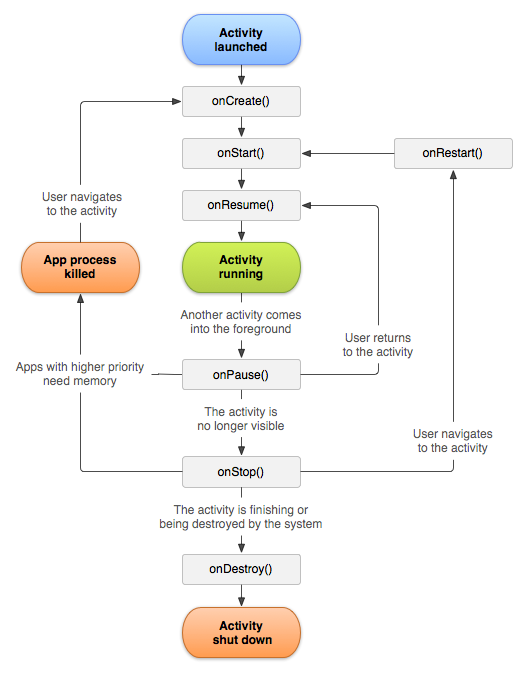
\includegraphics[width=0.9\textwidth]{img/activity_lifecycle.png}
    \caption{Lebenszyklus einer Activity \cite[]{androidDevDocu}}
    \label{Activity_Lifecycle}
  \end{centering}
\end{figure}
Im zweiten Szenario wird der Adressraum dieses Prozesses für andere Anwendungen benötigt (siehe Abbildung onStop() $\rightarrow$  onCreate()). Das Betriebssystem terminiert in Folge dessen den Prozess und damit auch alle darin laufenden Threads. Für die Nebenläufigkeit auf Thread Ebene würde dies bedeuten, dass alle Threads zusammen mit dem Prozess mit terminiert werden. Kommt die Anwendung durch den Aufruf des Nutzers wieder in den Vordergrund, so wird zunächst wieder ein Prozess mit entsprechendem Adressraum vom Betriebssystem eingerichtet, der UI Thread neu erzeugt und nun in dem UI Thread die Activity neu instanziiert (dabei Aufruf onCreate()). Alle zuvor erzeugen sekundären Threads existieren nicht mehr. Die Verarbeitung im Hintergrund wurde unterbrochen und terminiert. Die Hintergrundverarbeitung lässt sich ggf. neu aus der onCreate Methode heraus neu starten.

\section{Anforderungen an Applikationen}
Abschließend zu dieser Einführung in die grundlegenden Konzepte zur Ausführung und den Bestandteilen von Android Applikationen, werden nun allgemeine Anforderungen an die Applikationen zusammengefasst, wie sie auch der Application Style Guide von Google vor gibt.
Applikationen für das Android Betriebssystem verfügen zum großen Teil über eine graphische Benutzeroberfläche, die wenigsten sind reine Hintergrund Programme. Darum liegt auch der Fokus der Applikationen auf deren Benutzbarkeit. Entsprechend ergeben sich auch besondere Anforderungen für die Entwicklung von Nebenläufigkeit. In Android Applikationen wird die Interaktion mit dem Benutzer über den Hauptthread (= UI- Thread), abgehandelt. Sind nun innerhalb einer Applikation zeitintensive Berechnungen oder andere Vorgänge definiert, so ist darauf zu achten, dass dadurch nicht der UI-Thread blockiert wird. Dieser soll stets bereitgehalten werden um mit dem Benutzer zu interagieren. Eine nebenläufige Verarbeitung ist also so zu definieren, dass sekundäre Threads vom UI Thread aus initialisiert und gestartet werden können und im Weiteren völlig losgelöst vom UI Thread operieren. Kommt es zum Nachrichtenaustausch zwischen dem UI Thread und den sekundären Threads (Datenaustausch) darf dies für den UI Thread keine zeitaufwändige Operation darstellen, diese Nachrichten zu verarbeiten. Weiter benötigt der Nutzer auch im Einzelfall Rückmeldung über den Bearbeitungsstand aus den sekundären Threads, sowie auch im Fehlerfall entsprechende Meldungen.

\section{Fokus und Eingrenzung}
In dieser Arbeit soll sich primär darauf konzentriert werden, wie asynchrone Parallelverarbeitung realisiert werden kann und welche Gefahren sich aus der Komplexität dieser Aufgabe ergeben können. Weiter ist die Fragestellung im Fokus, wie eine Fehlerbehandlung innerhalb asynchroner Parallelverarbeitung realisiert werden kann bzw. wie unterschiedliche Meldungen an den UI -Thread übertragen werden können. Um die Problemstellung der asynchronen Parallelverarbeitung für Andorid Plattformen greifbarer zu machen werden zwei Szenarien beschrieben in denen man bei der Implementierung die asynchronen Parallelverarbeitung sinnvoll demonstrieren kann:
\paragraph{Zugriff auf Web Ressourcen} 
In Android Applikationen ist es häufig nötig auf Web Ressourcen zu zu greifen. Bis jedoch die gesamte Ressource geladen ist, kann es u.U. je nach Verfügbarkeit des Netzwerks zu längeren Wartezeiten kommen. Arbeitet die Applikation nun streng sequentiell, so würde sie blockieren, bis die Ressourcen geladen sind und sich dann damit zurückmelden.
\paragraph{Zeitintensive Berechnungen}
Neben dem Zugriff auf Netzwerkressourcen können auch einzelne Berechnungen oder Suchfunktionen längere Zeit in Anspruch nehmen. Ebenso ist hier auf eine asynchrone Parallelverarbeitung zu achten, denn genauso wie in o.g. Szenario kann hier die Anwendung bei sequentieller Abarbeitung blockieren (also keine Benutzereingaben verarbeiten) und in Folge dessen durch das Betriebssystem terminiert werden. 
\newline
Die im Kapitel 2 aufgeführten Implementierungsbeispiele beziehen sich primär auf das zweite Szenario, um für Präsentationszwecke unabhängiger von Netzwerkeigenschaften zu sein.


\chapter{Asynchrone Parallelverarbeitung unter Android}
Für die Realisierung von asynchroner Parallelverarbeitung werden in diesem Kapitel drei Lösungsansätze entwickelt. Jeder dieser Ansätze versucht die asynchrone Verarbeitung im Hintergrund, losgelöst vom Hauptthread der Applikation zu realisieren. Als Beispiel für die im Hintergrund zu tätigende Verarbeitung steht eine rechenintensive und damit zeitaufwändige mathematische Operation. Ziel ist mit dieser Operation ausreichend Rechenauslastung zu erzeugen, sodass im Falle einer synchronen Abarbeitung die Applikation blockieren kann.

\section{Bolckierung der Ein-/Ausgabe durch zeitintensive Verarbeitung}
Dieser Abschnitt soll einen Einblick in das Verhalten von Applikationen unter dem Android Betriebssystem geben, wenn zeitintensive Berechnungen durchgeführt werden. Das Implementierungsbeispiel ist an das in Kapitel 1.9 beschriebene Szenario zu zeitintensiven lokalen Berechnungen angelehnt.
Die folgende Abbildung zeigt zwei Fenster einer Android Applikation mit je einem Knopf zum Start einer bestimmten zeitintensiven mathematischen Berechnung, deren Ergebnisse auf im jeweiligen Fenster angezeigt wird.
\begin{figure}[H]
  \begin{centering}
    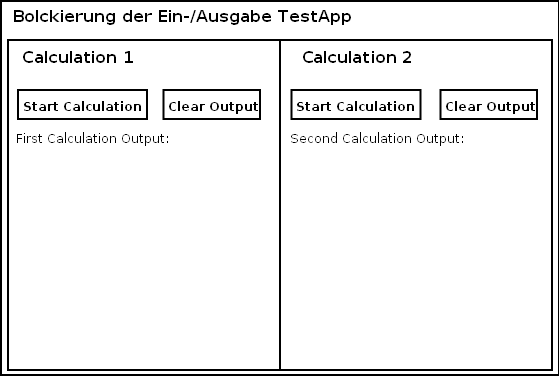
\includegraphics[width=0.9\textwidth]{img/BlockingIO_testApp_Mockup.png}
    \caption{Mockup zur Testapplikation: Blockierende Ein-/Ausgabe}
    \label{BlockingIO_testApp_Mockup}
  \end{centering}
\end{figure}
Die mathematische Operation ist so gestaltet, dass sie im Komplexitätsgrad variabel einstellbar ist und somit auch die Verarbeitungszeit verlängert werden kann. Dabei handelt es sich um die Berechnung einer Quersumme aus einer sehr großen Primzahl. Die Ermittlung der Primzahl verlängert sich in Abhängigkeit zu der im Die mathematische Operation ist so gestaltet, dass sie im Komplexitätsgrad variabel einstellbar ist und somit auch die Verarbeitungszeit verlängert werden kann. Dabei handelt es sich um die Berechnung einer Quersumme aus einer sehr großen Primzahl. Die Ermittlung der Primzahl verlängert sich in Abhängigkeit zu der im Vorhinein definierten Mindestgröße der Primzahl (hier 1500Byte BigInteger):\newline\newline
\texttt{BigInteger veryBig = new BigInteger(1500, new Random());\newline
BigInteger randomPrimeNumber = veryBig.nextProbablePrime();\newline
int summe = 0;\newline\newline
while (0 != randomPrimeNumber.compareTo(BigInteger.ZERO))\newline 
\{ \newline
       // addiere die letzte ziffer der uebergebenen zahl zur summe \newline
       summe = summe + (randomPrimeNumber.mod(BigInteger.TEN)).intValue(); \newline\newline\newline
       // entferne die letzte ziffer der uebergebenen zahl \newline
       randomPrimeNumber = randomPrimeNumber.divide(BigInteger.TEN); \newline
       \} \newline
targetString.append(summe);\newline
}
Die Berechnung wird dabei angestoßen aus der Activity und allein innerhalb des UI Thread durchgeführt. In einem ersten Versuch wird die Komplexität nach und nach erhöht um zunehmend die Interaktion der Applikation mit dem Nutzer über die Benutzerschnittstelle zu blockieren. Nach einer bestimmten Blockierungszeit T ist zu beobachten, das der ANR Dialog des Betriebssystems erscheint und anbietet die Applikation zu beenden oder weiter zu warten. An dieser Stelle registriert das Betriebssystem, dass der UI-Thread als Haupt-Thread der Applikation für die Zeit T keine weitere Interaktion des Benutzers verarbeiten kann. Der Benutzer ist bis zu diesem Zeitpunkt nach Aktivierung der Berechnung nicht in der Lage die Applikation zu beenden oder zu wechseln. Daher schreitet nun das Betriebssystem ein, pausiert die Applikation und bietet dem Nutzer in einem ANR-Dialog an, die Applikation zu terminieren, oder weiter auf die Rückmeldung der Applikation zu warten.

\section{Parallelverarbeitung mit der Java Standard Edition (Java Concurrency)}
In diesem Abschnitt wird versucht die zeitintensive Berechnung aus dem letzten Abschnitt, mittels der allgemeinen Mechanismen der Java Standard Edition in eine parallele Verarbeitung auszulagern. Damit soll das Blockieren der Anwendung verhindert werden. Hierzu wird die Berechnung in eine Klasse ausgelagert, die das Interface \texttt{java.lang.Runnable} implementiert. Diese kann daraufhin einem neuen Thread zur Ausführung übergeben werden. Der folgende Auszug aus dem Quellcode zeigt dabei den Konstruktor, sowie die \texttt{run()}- Methode der Klasse.\newline\newline\newline\newline\newline\newline
\texttt{
public RandomPrimeNumGenerator(final View aView, final Handler aCallbackHandler)\newline
\{ \newline
 Log.d(TAG,\grqq Call Constructor\grqq );\newline
 targetView = aView;\newline
 handler = aCallbackHandler;\newline
\} \newline
  @Override\newline
  public void run()\newline
  \{ \newline
     Log.d(TAG, \grqq Call run\grqq);\newline
       String result = startCalculation();\newline
       Message message = new Message();\newline
       Bundle bundle = new Bundle();\newline
       bundle.putCharArray(String.valueOf(targetView.getId()), result.toCharArray());\newline
       message.setData(bundle);\newline
       Log.d(TAG,\grqq Call handler\grqq );\newline
       handler.sendMessage(message);\newline
   \} \newline\newline
} \newline
Das hier verwendete Handler Objekt wird dem Konstruktor aus der Activity übergeben. Wird die durch den Konstruktor \texttt{RandomPrimeNumGenerator} erzeugte Runnableinstanz nun einem Thread Konstruktor übergeben und auf dieser Threadinstanz die \texttt{start()}- Methode Aufgerufen, so startet die Java Virtuelle Maschiene einen neuen Thread, der die zeitintensive Berechnungen ausführt. Der folgende Codeabschnitt ist in der Activity defininiert. Es wird somit aus dem Main Thread heraus ein neuer Thread erzeugt.\newline\newline\newline
\texttt{
private final Handler handler = new Handler();\newline\newline
public void initCalculation(View aView)\newline
  \{ \newline
     RandomPrimeNumGenerator runnable =
        new RandomPrimeNumGenerator(aView, handler);\newline\newline  
     Thread newThread = new Thread(runnable);\newline
     newThread.start();\newline
  \} \newline
} \newline
Die Händler Instanz, welche dem Konstruktor der Klasse \texttt{RadomPrimeNumGenerator} mitgegeben wurde, dient dabei der Kommunikation zwischen der Activity im UI-Thread und dem neuen Thread. So ist es möglich mittels einer Rückruf Methode, Informationen zurück an den UI-Thread zu spielen. Die Handler Implementierung stammt aus dem Packet android.os und ist demnach keine Funktionalität aus der Java Standard Edition. Es gibt alternativ auch andere Möglichkeiten mittels der Mechanismen aus der Java Standard Edition die Kommunikation zwischen den Threads zu realisieren. So kann eine eigene Nachrichteninfrastruktur geschaffen werden (vgl. Kapitel 1.x MessageQueue) oder es können auch Java Futures genutzt werden. Dennoch ist es für dieses Beispiel sinnvoll sich der Android-spezifischen Funktionalität zur Kommunikation über Thread Grenzen zu bedienen, denn diese wird bereits durch das Android Betriebssystem für jede Applikation bereitgestellt. Eine eigene Implementierung ist daher zwar jeder zeit möglich, stellt aber eine unnötige Redundanz dar. Diese Funktionalität wird im nächsten Abschnitt kurz erläutert um weiter auf deren korrekte Anwendung eingehen zu können.

\subsection{Handler-Looper Mechanismus zur Inter-Thread-Kommunikation}
Das Android SDK bietet für die Kommunikation zwischen Threads, die der selben Applikation angehören den Handler Looper Mechnismus an. Damit ist es möglich einen Thread an die applikationsinterne Nachrichteninfrastruktur einzuhängen und mit dem Haupt Thread, also hier dem UI Thread kommunizieren. Die Kommunikation ist dabei unidirektional. Hier gelangen Nachrichten nur von den sekundären Threads über die Nachrichtenstruktur zum UI-Thread und nicht umgekehrt. Die Nachrichtenstruktur wird in Form einer Nachrichtenwarteschlange umgesetzt (einer Instanz vom Typ MessageQueue), die nach dem First-In-First-Out-Prinzip durch ein Objekt vom Typ \texttt{android.os.Looper} abgearbeitet wird. Für die Instantiierung des Handlers gilt, dass er stets nur aus dem Thread erzeugt werden darf, der auch über eine valide Looper Instanz und somit über eine MessageQueue Instanz verfügt. Da in der Regel eine Looper Instanz bei Start einer Anwendung zusammen mit der entsprechenden MessageQueue innerhalb des UI-Threads erzeugt wird, bietet es sich an, den Handler ebenfalls hier zu initialisieren um Nachrichten an den UI-Thread zu übertragen.
\begin{figure}[H]
  \begin{centering}
    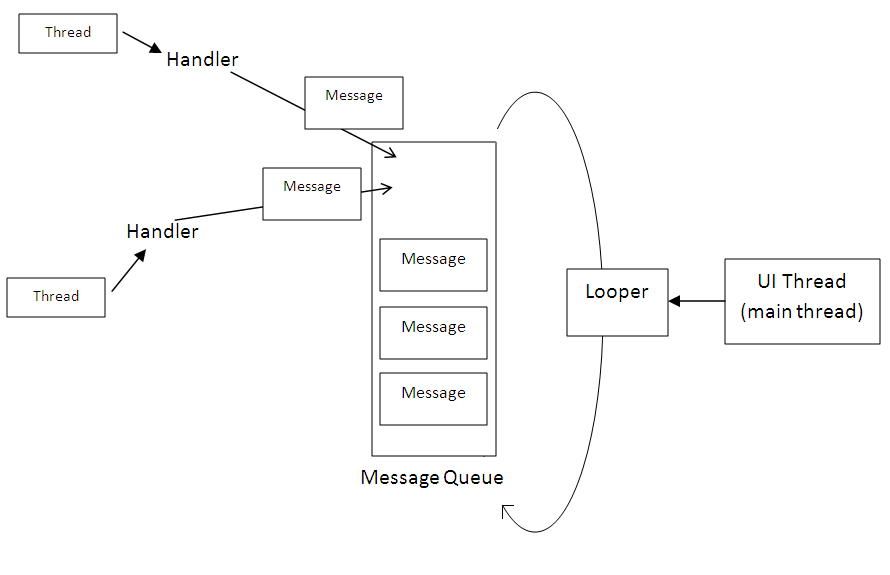
\includegraphics[width=1\textwidth]{img/handler_looper.png}
    \caption{Handler Looper Mechanismus für Android Applikationen \cite[]{handlerLooperBlock}}
    \label{handler_looper}
  \end{centering}
\end{figure}
Die o.g. MessageQueue und die Looper-Instanz wird zum Initialisierungszeitpunkt der Applikation erzeugt. Sie bildet über die Kommunikation zwischen sekundären Threads und dem UI Thread hinaus, auch die Kommunikation zwischen den Basiskomponenten der Applikation ab (siehe Kapitel 1.3.3 Komponentenmodell). Darunter zählen u.a. Activities, Broadcast Receivers, etc.

\subsection{Verwendung des Handler Looper Mechnismus }
In unserem Beispiel wird ein Handler aus der Activity erzeugt, die in dem UI-Thread verarbeitet wird. Der Hander kann somit in seinem Konstruktor auf die Looper Instanz des UI Threads zugreifen und damit auch die Referenz der MessageQueue abrufen, in die er Nachrichten ablegen soll. In der run()-Methode der Klasse RandomPrimeNumGenerator wird das Ergebnis der Berechnung als gebundenes Schlüssel-Wert-Paar in einem Nachrichtenobjekt vom Typ anroid.os.Message abgelegt und der Handlerinstanz als zu versendende Nachricht übergeben.\newline\newline
\texttt{
@Override\newline
public void run()\newline
  \{\newline
     Log.d(TAG, \grqq Call run\grqq);\newline
       String result = startCalculation();\newline
       Message message = new Message();\newline
       Bundle bundle = new Bundle();\newline
       bundle.putCharArray(String.valueOf(targetView.getId()),
                           result.toCharArray());
       message.setData(bundle);\newline
       Log.d(TAG,\grqq Call handler\grqq);\newline
       handler.sendMessage(message);\newline
 \}\newline
}\newline
Die Handlerimplementierung in der Activity liefert die Rückruf Methode \texttt{handleMessage()}, die der Looper aufruft, wenn er die Nachricht unserer Handlerinstanz aus der Nachrichtenschlange nimmt.\newline\newline
\texttt{ 
private static Handler HANDLER = new Handler()\newline
  \{\newline
     @Override\newline
     public void handleMessage(Message msg)\newline
     \{\newline
        updateView(msg);\newline
     \}\newline
  \};\newline
}\newline
Im Falle von mehreren Handlerinstanzen, die Nachrichten in die MessageQueue ablegen, gibt es keine Kontrolle über die Reihenfolge. Die Nachrichten werden durch den Looper in der Regel (abhängig von der MessageQueue Implementierung) nach dem First-In-First-Out-Prinzip abgearbeitet, welches für komplexere Handler – Thread Konstrukte (also mehr als ein sekundärer Thread) zu beachten ist. Die Methode \texttt{updateView(msg)} der Activity wird im weiteren Programmverlauf nun asynchron aufgerufen und extrahiert die Nutzdaten aus der übermittelten Nachricht, um damit die jeweiligen Interaktionselemente der Benutzerschnittstelle zu aktualisieren.\newline\newline
\texttt{ 
  public static void updateView(Message aMessage)\newline
  \{ \newline
     Log.d(\grqq RandomPrimeNumGenerator\grqq, \grqq Callback handleMessage\grqq);\newline
     Bundle bundle = aMessage.getData();\newline
\newline
     if(bundle.containsKey(String.valueOf(R.id.startCalculation1)))\newline
     \{\newline
        char[] firstResult = (char[])bundle.get(String.valueOf(R.id.startCalculation1));\newline
        Log.d(\grqq RandomPrimeNumGenerator\grqq, \grqq Callback view string: \grqq + String.valueOf(firstResult));\newline
\newline
        firstCalculationOutput.setText(String.valueOf(firstResult));\newline
        firstCalculationOutput.invalidate();\newline
    \}\newline
\newline
     if(bundle.containsKey(String.valueOf(R.id.startCalculation2)))\newline
     \{\newline
        char[] secondResult = (char[])bundle.get(String.valueOf(R.id.startCalculation2));\newline
        Log.d(\grqq RandomPrimeNumGenerator\grqq, \grqq Callback view string: \grqq +                                                                                                                                                                 
      String.valueOf(secondResult));\newline\newline
        secondCalculationOutput.setText(String.valueOf(secondResult));\newline
        secondCalculationOutput.invalidate();\newline
     \}\newline
  \}\newline
}\newline
\subsection{Probleme bei der Nutzung des Handler Looper Mechanismus}
Das den letzten Abschnitten vorgestellte Implementierungsbeispiel zur Java Concurrency zeigt, wie Parallelverarbeitung mit der Standard Thread Erzeugung aus der Java SE Paket realisiert werden kann. Jedoch besteht so wie der Handler Looper Mechnismus hier verwendet wird ein Risiko. Dadurch, dass der UI-Thread eine Handler Instanz erzeugt und diese dann im sekundären Thread genutzt wird, können Memory Leaks (Speicherlecks) entstehen die, die Stabilität des Systems gefährden können. Innerhalb von Applikationen unter Android werden in der Regel für bestimmte Ereignisse wie z.B. Konfigurationsänderungen (Drehen des Bildschirm = Veränderung des Darstellungsformates) die betreffenden Activities neu instantiiert und die alten Instanzen dem Garbage Collector übergeben. Die Folgende Graphik skizziert die Abhängigkeiten bei einem möglichen Implementierungsszenario:
\begin{figure}[H]
  \begin{centering}
    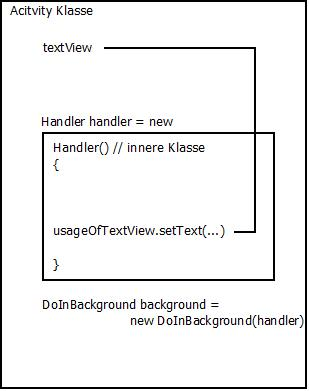
\includegraphics[width=0.7\textwidth]{img/weakReference.jpeg}
    \caption{Speicherleck durch non-static Handler Implementierung sowie falsche Referenzierung von Objekten der äußeren Klasse in der innerer Klasse}
    \label{weakReference}
  \end{centering}
\end{figure}
In diesem Fall kann die alte Activity Instanz nicht entsorgt werden, da diese immer noch eine Referenz auf das aktuell in einem zweiten Thread genutzte Handler Objekt hält. Zusätzlich wird innerhalb der Handler Klasse auf ein Element der Activity zugegriffen(\texttt{textView}). Beide Referenzen hindern den Garbage Collector daran die Activity abzuräumen, solange die Verarbeitung im sekundär Thread noch läuft. Dauert die Hintergrundverarbeitung nun sehr lange, so ist es durch häufiges Drehen des Displays schnell möglich, weitere Activity Instanzen zu erzeugen und somit das System zu destabilisieren (der Hauptspeicher läuft voll). Dieser Effekt wird noch dadurch verstärkt, dass gerade die Activity alle GUI Elemente referenziert, also sehr speicherintensiv ist. Der Konstruktor der Klasse android.os.Handler versucht bereits zur Instanziierung den Entwickler vor diesem Risiko zu warnen:\newline
\texttt{ \newline
   public Handler() \{\newline
     if (FIND\_POTENTIAL\_LEAKS) \{ \newline
           final Class<? extends Handler> klass = getClass();\newline
           if ((klass.isAnonymousClass() || klass.isMemberClass() || klass.isLocalClass()) \&\& 
                 (klass.getModifiers() \& Modifier.STATIC) == 0) \{\newline
               Log.w(TAG, \grqq The following Handler class should be static or leaks might occur: \grqq +
                   klass.getCanonicalName());\newline
           \}\newline
       \}\newline
\newline
       mLooper = Looper.myLooper();\newline
       if (mLooper == null) \{\newline
           throw new RuntimeException(
               \grqq Can't create handler inside thread that has not called Looper.prepare()\grqq);\newline
       \}\newline
       mQueue = mLooper.mQueue;\newline
      mCallback = null;\newline
   \}\newline
}\newline
Hier wird deutlich, dass explizit geprüft wird, ob das Handler Objekt als statisches Objekt aus einer inneren Klasse heraus deklariert wurde. Falls nicht wird schon hier eine Warnung ausgegeben, dass an dieser Stelle ein Speicherleck droht:\newline
\texttt{Log.w(TAG, \grqq The following Handler class should be static or leaks might occur: \grqq +
               	class.getCanonicalName());}\newline
Für die Handler Referenz würde somit schon die Definition als statische Instanz ausreichen. Werden jedoch dem Sekundär-Thread weitere Referenzen übergeben, so sind diese als \texttt{java.lang.ref.WeakReferences} zu kapseln. Diese zeigen dem Garbage Collector an, dass er bei der Evaluation z.B. einer Activity Instanz nicht die aktuelle Nutzung von \texttt{WeakReferenzes} untersuchen muss.

\subsection{Vorsicht im Umgang mit Java Futures}
Als Nachtrag zu dem Implementierungsbeispiel aus dem letzten Abschnitt, wird auf die berechtigte Fragestellung eingegangen, ob nicht auch Java Futures für den Informationsaustausch, bzw. die Ergebnisübergabe genutzt werden können anstatt sich dem Handler Looper Mechanismus zu bedienen. Java Futures bieten zwar grundsätzlich die Möglichkeit asynchrone Verarbeitung zu realisieren, jedoch eignen sie sich in diesem Anwendungszenario eher weniger für den Austausch von Nachrichten bzw. Rückgabe des Ergebnisses aus der Hintergrundberechnung. Denn wird für den Erhalt eines Ergebnisses vom UI Thread Future.get() aufgerufen so, wird der UI Thread durch die get()-Methode blockiert, solange das angeforderte Ergebnis noch nicht vorliegt. Dies ist gerade das Verhalten was verhindert werden muss. Alternativ kann ein Konstrukt entworfen werden, in der kontinuierlich oder in bestimmten Zeitabständen versucht wird das Ergebnis abzufragen, doch diese Lösung ist weder elegant noch performant. Entsprechend eignet sich die Java Standart Implementierung des Future eher weniger für die in dieser Arbeit fokussierten Problemstellung. 

\section{Parallelverarbeitung mit AndroidAsyncTask (Anroid Concurrency)}
Im Vorangegangenen Abschnitt wurde gezeigt, das die Realisierung mittels Java Concurrency und dem Handler Looper Konstrukt durchaus einen gewissen Komplexitätsgrad und damit auch einige Gefahren für eine stabile Anwendung birgt. In diesem Abschnitt wird ein Konzept von Google vorgestellt, welches die Realisierung von nebenläufiger Verarbeitung deutlich vereinfachen soll. Der Schlüssel hierzu ist die abstrakte Klasse android.os.AsyncTask. Sie stellt eine Hilfsklasse zu dem oben beschriebenen Handler Looper Mechanismus dar und muss für die Verwendung abgeleitet werden. Dabei sind drei generische Primärparametertypen zu definieren, welche die  Nutzdatentypen zur Initialisierung, Durchführung, und Ergebnisrückgabe der Hintergrundberechnung konkretisieren.\newline
\newline
\texttt{private class AsyncTaskImpl extends AsyncTask<Params, Progress, Result>}
\newline
Für Parametertypen gilt:
\begin{itemize}
\item Params $\rightarrow$ betrifft alle Parameter, die Nutzdaten für die Hintergrundverarbeitung enthalten. Sie werden zum Ausführungszeitpunkt mittels der Methode \texttt{doInBackground(Params… params)} übertragen.
\item Progress $\rightarrow$ betrifft alle Parameter, die während der Ausführung mittels der Rückruf Methode \texttt{onPublishProgress(Progress… progress)} den Fortschritt, bzw.  den Status der Hintergrundverarbeitung an den UI-Thread transportieren.
\item Result $\rightarrow$ betrifft alle Parameter, die das Ergebnis aus der Hintergrundverarbeitung mittels der Rückruf Methode \texttt{onPostExecute(Result …result)} an den UI-Thread übergeben.
\end{itemize}
Die Android Developper Dokumentation nennt weiter die vier wesentlichen Methoden zur Steuerung der Hintergrundverarbeitung:
\begin{itemize}
\item \texttt{onPreExecute()}
\item \texttt{doInBackground(Params…params)}
\item \texttt{onProgessUpdate(Progress… progress)}
\item \texttt{onPostExecute(Result… result)}
\end{itemize}
Die Methoden teilen das Ausführungsmodell der Verarbeitung im AsynchTask in klar voneinander abgetrennte Abschnitte (siehe auch Sequenzdiagramm in Abbildung 10). Die Methodennamen geben einen ersten Hinweis auf die jeweiligen Aufrufzeitpunkte, die in der Klasse AsyncTask fest definiert sind. So wird die Methode\newline 
\texttt{\newline
onPreExecute()\newline
}\newline
vor der Hintergrundverarbeitung bereits im Konstruktor der Klasse AsyncTask aufgerufen. Hier kann entsprechend alle Logik integriert werden, die noch vor der eigentlichen Hintergrundverarbeitung stattfinden soll. Der hier definierte Code wird noch auf dem UI-Thread ausgeführt. Dies bietet sich an für Initialisierungen wie z.B. für eine Prozessanzeige.\newline
Die Methode\newline \newline
\texttt{doInBackground()}\newline\newline
ist als abstrakte Methode gekennzeichnet und muss bei der Vererbung von AsyncTask überschrieben werden. Sie kapselt die aufzurufende Logik um diese in einem separaten Thread aufrufen zu können. In unserem Beispiel wird hier die zeitintensive Berechnung definiert. Die \texttt{doInBackground()}-Methode ist eine Rückruf-Methode und wird indirekt angestoßen durch den Aufruf\newline 
\texttt{\newline
asyncTaskInstance.execute(Params…params)\newline
}\newline
Die Klasse \texttt{AndroidAsyncRandomPrimeGen} überschreibt die \texttt{doInBackground()}-Methode und integriert hier die zeitintensive Verarbeitung:\newline
\texttt{\newline
@Override\newline
  protected AsyncTaskResult<String> doInBackground(Integer... params)\newline
  \{\newline
     if(params == null || params.length != 1)\newline
    \{\newline
        return new AsyncTaskResult<String>(new IllegalArgumentException(\grqq Not the rights params:\grqq + params));\newline
    \}\newline
     triggerViewId = params[0].intValue();\newline
\newline
     StringBuilder targetString = new StringBuilder(10);\newline
     for(int i = 0; i < 10; i++)\newline
    \{\newline
\newline
BigInteger veryBig = new BigInteger(1500, new Random());  //Zeitintensive Berechnung \newline
           //siehe Bsp BlockierendeEingabeAusgabe...\newline
     return new AsyncTaskResult<String>(targetString.toString());\newline
 \}\newline
}\newline
Die oben beschriebenen Übergabeparametertypen werden in diesem Codebeispiel zur Methode \texttt{doInBackground()} als Integer konkretisiert und spezifizieren in der Implementierung die ID der View, welche die Berechnung angestoßen hat. An Hand dessen wird später die Ziel-View ermittelt, die das Ergebnis darstellen soll. Das Ergebnis der Berechnung wird hier als konkreter \texttt{AsyncTaskResult<String>} Typ zurückgegeben, damit dieser String an die \texttt{onPostExecute(Result … result)} Methode weitergegeben werden kann. Analog zur Hintergrundverarbeitung bietet Google mit der Methode \texttt{onProgressUpdate()} die Möglichkeit aus der laufenden Berechnung im sekundären Thread, Informationen oder Nachrichten wie z.B. Statusmeldungen an den UI Thread zu senden. Die Methode \texttt{onPostExecute()} wird nach Abschluss der Hintergrundoperationen dann wieder auf dem UI-Thread ausgeführt. Sie bietet sich an, um finale Aktualisierungen auf Basis der Ergebnisse aus der Hintergrundverarbeitung durchzuführen. In unserem Beispiel könnte das Ergebnis in die jeweiligen View Objekte der Activity übertragen werden:\newline
\newline
\texttt{@Override\newline
   protected void onPostExecute(AsyncTaskResult<String> result) \{\newline
...\newline
           //update user interface\newline
           String realResult = result.getResult();\newline
\newline
           if (triggerViewId == R.id.startCalculation1) \{\newline
               firstOutputView.setText(realResult);\newline
               firstOutputView.invalidate();\newline
           \}\newline
           if (triggerViewId == R.id.startCalculation2) \{\newline
               secondOutputView.setText(realResult);\newline
               secondOutputView.invalidate();\newline
           \}\newline
       \}\newline
}
Da einzig und allein von den vorgestellten Methoden, die \texttt{doInBackground()} Methode in dem sekundären Thread ausgeführt wird, muss darauf geachtet werden, keine zeitintensive Logik in den anderen Methoden zu integrieren. Ansonsten besteht wieder die Gefahr der blockierenden Anwendung, analog zu der Beispielimplementierung in Kapitel 2.1. Weiter ist gemäß der Android Developer Dokumentation darauf zu achten, dass nur gering zeitaufwändige (wenige Sekunden) Operationen mittels des AsyncTask in eine Hintergrundverarbeitung ausgelagert werden sollten. Woran das liegt und welche Konsequenzen sich aus längeren Operationen ergeben wird hier nicht genannt. Die Android Developper Dokumentation gibt hierzu lediglich einen groben Überblick wie dieser Mechanismus optimal zu nutzen ist und für welche Problemstellungen sich die Verwendung der Klasse AsyncTask eignet. Es bleiben also weitere Fragen offen:
\begin{itemize}
\item Wie funktioniert nun der AsyncTask Mechanismus konkret?
\item Gemäß der Dokumentation wird die Inter-Thread Kommunikation mittels des oben vorgestellten Handler-Looper Mechanismus (siehe auch Parallelverarbeitung mit Java SE) realisiert. Doch wie wird diese Kommunikation im Detail für die genannten Rückrufmethoden über Thread Grenzen hinaus umgesetzt? Wie wird zwischen Statusmeldungen und Ergebnismeldungen unterschieden?
\item Wie und wann wird der Hintergrund Thread erstellt?
\item Wie funktionieren die Executor Instanzen insbesondere der \texttt{THREAD-POOL-EXECUTOR} der in der Android Developper Dokumentation lediglich kurz genannt wird?
\end{itemize}
Diesen Fragen widmet sich der folgende Abschnitt in dem genauer auf die konkrete Implementierung der Klasse andorid.os.AsyncTask eingegangen wird.

\subsection{Ausführungsmodell von Android AsyncTask in Bezug auf Multi Threading}
Im letzten Abschnitt wurde auf die allgemeine Funktionsweise der Klasse android.os.AsyncTask eingegangen, ohne genauer zu hinterfragen wie die einzelnen Mechanismen im Hintergrund funktionieren. Dabei blieben noch einige Fragen offen, deren Klärung nun ein genauerer Blick in die Implementierung der abstrakten Klasse AndroidAsyncTask erfordert. In einem ersten Schritt wird zunächst das Ausführungsmodell gemäß der im letzten Abschnitt vorgestellten Beispielimplementierung im Detail vorgestellt. Hierzu dient das folgende Sequenzdiagramm:
\begin{figure}[H]
  \begin{centering}
    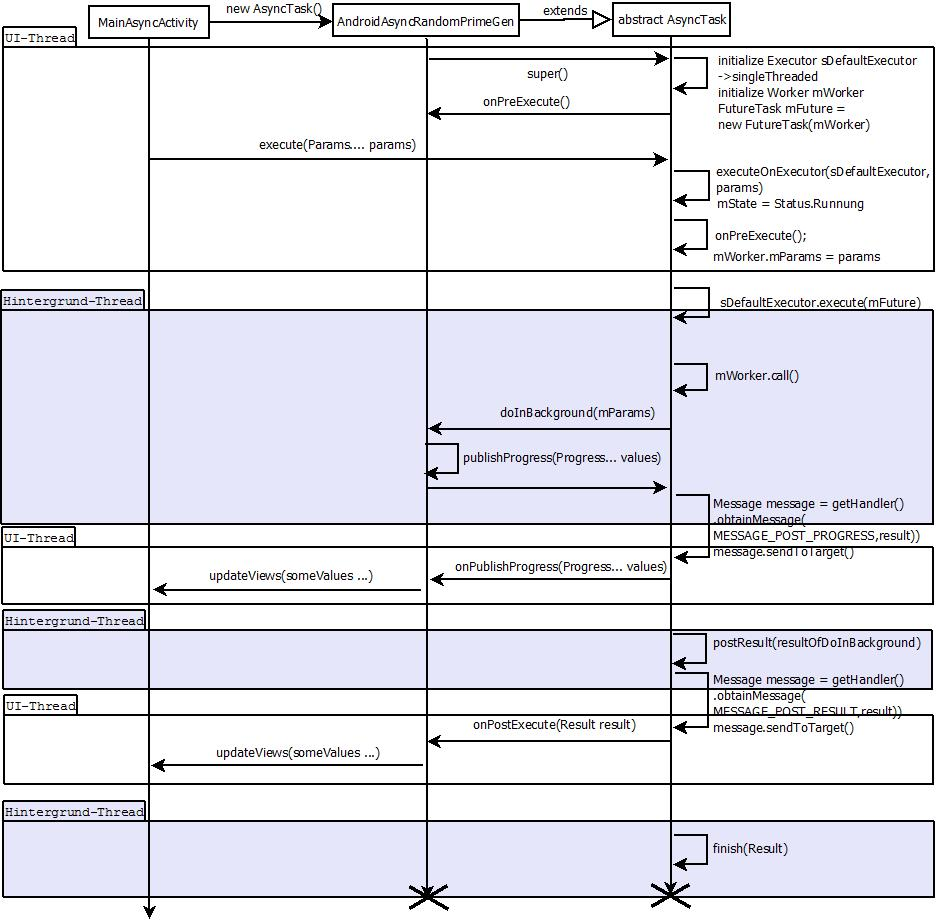
\includegraphics[height=1\textwidth]{img/asyncTask_seqenzdiagramm.png}
    \caption{Sequenzdiagramm zum internen Ablauf in Android AsyncTask mit Zuordnung zum jeweiligen Thread}
    \label{asyncTask_seqenzdiagramm}
  \end{centering}
\end{figure}
Das dargestellte Sequenzdiagramm gibt einen ersten Einblick in die interne Funktionsweise der Klasse AsyncTask. Es ordnet die einzelnen Vorgänge zur Initialisierung, Durchführung und Beendigung der Hintergrundberechung im Android AsycnTask dem jeweiligen Thread zu.  Es ist zu entnehmen, dass die Initialisierungen durch den Aufruf des Konstruktors angestoßen werden und im UI-Thead stattfinden. Zu diesen Initialisierungen gehören:\newline
\begin{itemize}
\item Erzeugung der Standart Executor Instanz, die die Ausführung in Thread steuert
\item Erzeugung einer Worker Instanz, welche die Hintergrundverarbeitung kapselt
\item Erzeugung einer Queue Instanz welche die später zu verarbeitenden Aufgaben hintereinander anreiht
\item Erzeugung eines Handlers der die asynchrone Kommunikation zwischen dem Hintergrund Thread und dem UI Thread gemäß des Handler Looper Mechanismus (siehe Abschnitt zu Handler Looper Mechanismus Kapitel 2.x) regelt.
\end{itemize}
Wird nun die \texttt{execute(Runnable r)} Methode des AsyncTask aufgerufen besteht noch die Möglichkeit weitere Initialisierungen in der Rückrufmethode \texttt{onPreExecute()} zu definieren. Auch dieser Aufruf wird noch durch den UI Thread verarbeitet. Erst mit dem Aufruf 
\texttt{sDefaultExecutor.execute(runnable);} wird die Hintergrundberechnung eingeleitet. In dem jeweils erzeugten Thread wird weiter durch eine Worker Instanz die Rückrufmethode \texttt{doInBackground()} aufgerufen, in der die zeitintensive Verarbeitung implementiert ist. Sollen hieraus nun Statusmeldungen, Zwischenergebnisse oder sonstige Daten noch während der Berechnung im HintergrundThread an den UI Thread übermittelt werden, kommt der in Kapitel 2.2 vorgestellte Handler Looper Mechanismus zur Anwendung. Die Nutzdaten werden der Methode \texttt{publishProgress(Params...params)} übergeben. Diese werden weiter in eine Handler Message gepackt, welche über den Schlüssel \newline
\texttt{private static final int MESSAGE\_POST\_PROGRESS = 0x2;}\newline
verfügt. Damit ist es möglich in der Handler-Implementierung die Daten des Message Objektes exakt an die richtigen Rückrufmethoden weiter zu leiten. Die Message wird der MessageQueue übergeben und der Hintergrund Thread fährt mit seiner Verarbeitung fort. Gemäß den Erläuterungen zum Handler Looper Mechanismus ruft der Looper im UI-Thread, wenn er das Message Objekt aus der Queue nimmt, die spezifische Handler Implementierung auf, extrahiert die Nutzdaten und sendet diese in Abhängigkeit zum Message Schlüssel an die jeweilige Rückrufmethode. Siehe hierzu die Handler Implementierung der Klasse AsyncTask:\newline
\texttt{\newline
private static class InternalHandler extends Handler \{\newline
\newline
@SuppressWarnings({\grqq unchecked\grqq, \grqq RawUseOfParameterizedType\grqq})\newline
@Override\newline
public void handleMessage(Message msg) \{\newline
AsyncTaskResult result = (AsyncTaskResult) msg.obj;\newline\newline
switch (msg.what) \{\newline
case MESSAGE\_POST\_RESULT:\newline
// There is only one result\newline
result.mTask.finish(result.mData[0]);\newline
break;\newline
case MESSAGE\_POST\_PROGRESS:\newline
result.mTask.onProgressUpdate(result.mData);\newline
break;\newline
\}\newline
\}\newline
\}\newline
}\newline
Analog findet die Übergabe des Ergebnisses der Hintergrundberechnung aus dem sekundären Thread in den UI-Thread statt. Dabei wird mittels der Methode \texttt{postResult(resultOfDoInBackground)} die Nachricht erzeugt und versandt. Der Handler erkennt an Hand des Nachrichteschlüssels:\newline
\texttt{private static final int MESSAGE\_POST\_RESULT = 0x1;}\newline
die entsprechende Rückrufmethode für die Nachrichten Verarbeitung im UI Thread :\newline
\texttt{onPostExecute(Result...result)}.\newline
Final wird der Status im Hintergrund Thread auf den Status \glqq Beendet\grqq gesetzt und dieser terminiert. Die Handler Instanz, welche spezifisch für diesen Thread erzeugt wurde, wird zusammen mit evtl. weiteren nun nicht mehr verwendeten Objekt Instanzen dem Garbage Collector übergeben.

\subsection{Serielle Ausführung in Android AsyncTask}
Wir haben bisher gesehen, wie das Ausführungsmodell der Klasse Android AsyncTask die Hintergrundverarbeitung in klar von einander getrennte Verarbeitungsschritte unterteilt und diese dem jeweiligen Thread zuordnet. Auch wurde deutlich, wie die Kommunikation Mittels des Handler Looper Mechnismus über Thread Grenzen hinaus realisiert ist. Es bleibt nun noch die Frage, wie die Berechnungen letzt endlich in einem neuen Thread ausgelagert werden. Damit verbunden ist die Frage nach der Funktionsweise der in der Android Developer Dokumentation grob skizzierten Executor Instanzen.
\begin{itemize}
\item DefaultExecutor $\rightarrow$ Serielle Ausführung
\item ThreadPoolExecutor $\rightarrow$ Parallele Ausführung
\end{itemize}
Gemäß der Dokumentation haben wir in dem Prototyp den DefaultExecutor verwendet und werden zunächst die Funktionsweise der seriellen Ausführung analysieren. Sieht man sich den initialen Aufruf der Hintergrundverarbeitung an, so stellt folgende Methode den Einstiegspunkt in die Verarbeitung durch AsyncTask dar:\newline
\texttt{\newline
public final AsyncTask<Params, Progress, Result> execute(Params... params) \{\newline
    return executeOnExecutor(sDefaultExecutor, params);\newline
\}\newline
}\newline
Darin wird der Aufruf an eine spezifische \texttt{executeOnExecutor()} Methode weitergeleitet und die zu verwendende Executor Instanz spezifiziert:\newline
\texttt{\newline
private static volatile Executor sDefaultExecutor = SERIAL\_EXECUTOR;\newline
}\newline
Dabei handelt es sich nach Android Developer Dokumentation um einen Executor, der die abzuarbeitenden Tasks seriell in einem sekundären Thread abarbeitet. Er stellt somit den Gegensatz zu der Executor Instanz THREAD-POOL-EXECUTOR dar, die es ermöglicht die Hintergrundverarbietung auf mehrere Threads zu verteilen. Jedoch wird von der Verwendung des THREAD-POOL-EXECUTOR in der Dokumentation abgeraten, da sich hier Probleme aus der nicht vorhersagbaren Reihenfolge der Abarbeitung und der Synchronisation von Ergebnissen ergeben können. Sieht man sich jedoch nun die Implementierung des empfohlenen SerialExecutors an, so erscheint es zunächst überraschend, dass sich dieser seinerseits des ThreadPoolExecutors bedient (siehe \texttt{scheduleNext()} Methode):\newline
\texttt{\newline
private static class SerialExecutor implements Executor \{\newline
    final ArrayDeque<Runnable> mTasks = new ArrayDeque<Runnable>();\newline
    Runnable mActive;\newline
\newline
    public synchronized void execute(final Runnable r) \{\newline
        mTasks.offer(new Runnable() \{\newline
            public void run() \{\newline
                try \{\newline
                    r.run();\newline
                \} finally \{\newline
                    scheduleNext();\newline
                \}\newline
            \}\newline
        \});\newline
        if (mActive == null) \{\newline
            scheduleNext();\newline
        \}\newline
    \}\newline
        protected synchronized void scheduleNext() \{\newline
        if ((mActive = mTasks.poll()) != null) \{\newline
            THREAD\_POOL\_EXECUTOR.execute(mActive);\newline
        \}\newline
    \}\newline
\}\newline
}\newline
Das folgende Aktivitätsdiagramm visualisiert den oben definierten Programmablauf um diesen besser zu verstehen. Es zeigt wie der Serial-Executor zur Initialisierung eine Queue erzeugt, in der die einzelnen abzuarbeitenden Aufgaben temporär vor deren Verarbeitung abgelegt werden.
\begin{figure}[H]
  \begin{centering}
    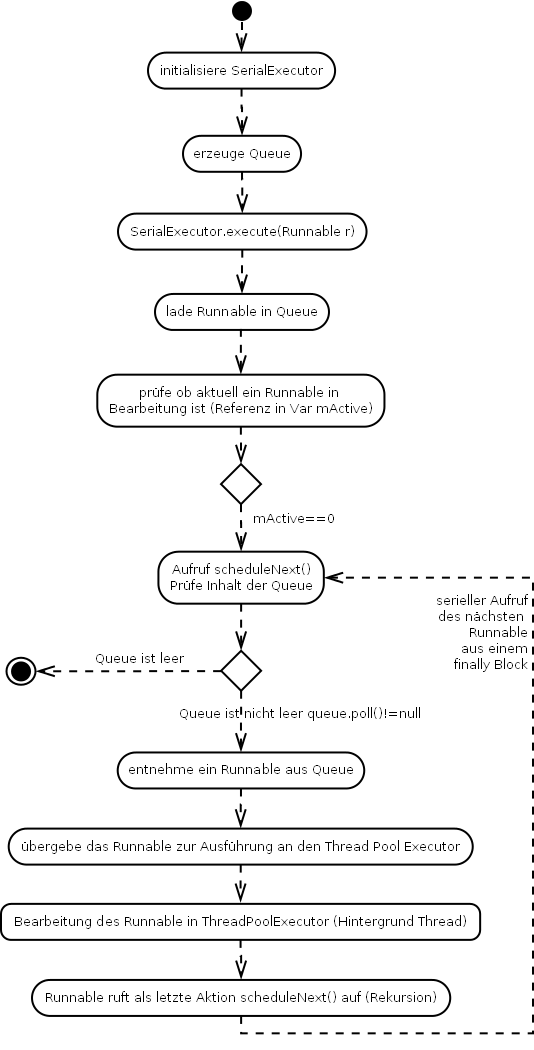
\includegraphics[width=0.7\textwidth]{img/ActivitydiagrammAsyncTaskSerialExecutor.png}
    \caption{Aktivitätsdiagramm zum SerialExecutor in Android AsyncTask}
    \label{ActivitydiagrammAsyncTaskSerialExecutor}
  \end{centering}
\end{figure}
Wird die \texttt{execute(Runnabel r)} - Methode des SerialExecutors aufgerufen, so wird die darin mit übergebene Runnable Instanz in der Queue abgelegt. Die folgende Prüfung, ob bereits ein Runnable in Bearbeitung ist ( z.B. durch aktuell laufende Verarbeitungen), stellt den Eintrittspunkt in die serielle Verarbeitung dar. Denn nur wenn sich aktuell keine Runnable Instanz in Bearbeitung befindet, wird eine neue Verarbeitung angestoßen. Den Start der Verarbeitung eines Runnabels definiert die Methode \texttt{schaduleNext()}. Darin wird ein Runnable aus der Queue genommen, und der Instanz vom Typ \texttt{ThreadPoolExecutor} zur Ausführung übergeben. Ist die Verarbeitung eines Runnables abgeschlossen, so wird rekursiv erneut die \texttt{schaduleNext()} - Methode aufgerufen und eine neue Verarbeitung gestartet. Dies wiederholt sich solange, wie zu verarbeitende Aufgaben, als Runnables aus der Queue genommen werden können.  Dem ThreadPoolExecutor, welcher für die parallele Ausführung von Runnabels in unterschiedlichen Threads gedacht ist, wird somit immer nur pro Verarbeitungszyklus ein Runnable zur Verarbeitung übergeben. Ist die Queue leer terminiert die Verarbeitung. Der SerialExecutor ist somit nichts weiter als ein Portionierer, der lediglich einen Task zur selben Zeit für die Bearbeitung durch den ThreadPoolExecutor frei gibt.\newline
Wird eine parallele Verarbeitung benötigt, kann direkt der ThreadPoolExecutor verwendet werden indem ihm n-Tasks zur Ausführung übergeben werden. Dieser verteilt die Tasks auf die von ihm verwalteten Threads. Die Reihenfolge der Abarbeitung ist jedoch damit nicht mehr kontrollierbar und genau vor diesem Szenario wird in der Andorid Developper Dokumentation gewarnt. Weiter kann es zu fehlerhaften Verhalten bei unkorrekt synchronisierten geteilten Zugriffen kommen.\newline
Die Android Developper Dokumentation nennt weiter zum AsyncTask in der empfohlenen Konfiguration mit dem Standart (Serial) Executor den Hinweis, dass sich dieser Mechanismus lediglich für Hintergrundverarbeitungen anbietet, welche generell wenig Zeit in Anspruch nehmen. Dies ist dem Design des AsyncTask geschuldet, der in der o.g. Variante lediglich einen Thread erlaubt. Für die Verarbeitung von mehreren Aufgaben, die jede für sich wenig Zeit benötigt, würde bei einer hohen Anzahl von Aufgaben, die Verarbeitung in der Summe aller Aufgaben deutlich länger dauern, als bei der parallelen Verarbeitung. Google ist sich über diese Problematik durchaus bewusst und gibt eben genau für dieses Anwendungsszenario, die Möglichkeit des ThreadPoolExecutors mit. Dabei hat das Design des Andorid AsyncTask über die unterschiedlichen Android Versionen immer wieder Änderungen erfahren. So hat sich die erste Version des AsyncTask Mechanismus generell auf die serielle Verarbeitung in einem Hintergrund Thread konzentriert. Mit der im September 2009 veröffentlichten Android Version 1.6 (Donut) änderte sich das Ausführungsmodell in Richtung einer parallelen Ausführung in einem ThreadPool, wie es der ThreadPoolExecutor ermöglicht. Ab der Android Version 3.0 (Honeycomb) hat Google sich für die sichere Variante entschieden und bietet wie oben vorgestellt im Standard die serielle Verarbeitung an, um die Schwierigkeiten und Risiken für die Applikationsentwicklung zu verringern. Damit ist diese Funktionalität auch für weniger erfahrene Entwickler leicht anwendbar.


\section{Parallelverarbeitung mit RXJava}
Die letzten Abschnitte haben gezeigt, wie mittels der Techniken aus unterschiedlichen Software Developper Kits Nebenläufigkeit in Android Applikationen realisiert werden kann. Dabei beschränken sich die Beispiele auf die imperative Programmierung. Mit dem Framework RXJava wird die Konzeption von Nebenläufigkeit nun aus deklarativer Sicht betrachtet. Wie sich dies auf unsere konkrete Problemstellung auswirkt wird im folgenden untersucht.
\subsection{Imperative und Deklarative Programmierung}
\paragraph{Imperative Programmierung} bezeichnet ein Programmierparadigma, bei dem Applikationen aus einer Abfolge von Befehlen definiert werden. Diese verändern Werte in gespeicherten Variablen und erzeugen innerhalb einer Verarbeitung die Ergebnismenge in einer vom Entwickler vorgegebenen Reihenfolge. Dabei werden entsprechend der vom Programm zu erledigenden Aufgabe die einzelnen Verarbeitungsschritte mittels konkreten Ausführungsanweisungen an den Rechner vorgegeben. Hier liegt der Fokus also darauf was in welcher Reihenfolge berechnet wird. Die imperative Programmierung ist das klassische und am weitesten verbreitete Paradigma. Dem gegenüber steht die deklarative Programmierung.

\paragraph{Deklarative Programme} stellen eher \glqq abstrakte\grqq Problembeschreibungen dar, in denen die Beschreibung, wie die Berechnung des Problems stattfinden soll im Vordergrund steht. Aufeinander folgende Ausführungsanweisungen an den Rechner sollen im Idealfall hier eher vermieden werden. Es kommt bei dieser Form der Programmierung also nicht auf den Ablauf oder das Halten von Zuständen an, sondern eher auf die Problemspezifikation selbst. Damit einher geht ein im Vergleich zur imperativen Programmierung relativ hoher Abstraktionsgrad. Dies kann zum Vorteil werden, wenn daraus kürzere und prägnantere Programme entstehen. In Bezug auf die Konzeption von Nebenläufigkeit, wie sie in dieser Arbeit thematisiert ist, bietet die deklarative Programmierung die Eigenschaft der sog. impliziten Parallelität. Damit ist gemeint, dass die abstrakte Form der Programmierung es begünstigt, die Auswertung von unabhängigen Programmteilen parallel durchzuführen. Eine weitere Erleichterung bei der Konzeption von Nebenläufigkeit bietet die deklarative Programmierung dadurch, dass bereits innerhalb von Problemstellungen enthaltene Parallelität nicht künstlich in sequentielle Abläufe überführt werden muss.\cite[vgl. S.5 ff.]{declarativProgrammingScript} 
\paragraph{Funktionale Programmierung} ist eine konkrete Ausprägung der deklarativen Programmierung. In der funktionalen Programmierung wird das Problem als Satz von Funktionen ausgedrückt. Funktionen repräsentieren die ausführbare Funktionalität. Funktionen können anderen Funktionen übergeben werden können ("code-as-data"). Des weiteren können die Funktionen kombiniert, verkettet oder manipuliert werden. In der reinen Form der funktionalen Programmierung werden keine Zustände in Form von Daten gehalten oder Zwischenergebnisse verwaltet. Stattdessen werden im Idealfall stets neue Daten erzeugt.\cite[]{funcProgrJava}   

\subsection{Reaktive Programmierung \& Reactive Manifesto}
Die ersten Ideen zum deklarativen Paradigma wurden bereits um 1930 mit dem Lamda Kalkül von Alonso Church formuliert. Obwohl dieses Paradigma bereits lange bekannt ist erlebt es aktuell wieder eine große Aufmerksamkeit in der Welt der Softwareentwicklung. Eine Begründung findet sich in der zur Zeit fokussierten reaktiven Programmierung. Reaktive Programmierung ist eine weitere Ausprägung der deklarativen Programmierung. Sie ist darauf spezialisiert asynchrone Verarbeitung als Datenströme einer Anwendung zu beschreiben. Zu diesen Strömen kann sich ein sog. \glqq Subscriber\grqq registrieren, also ein Abonnement anlegen und je nach Bedarf unterschiedliche Operationen darauf ausführen. Die Ströme können dabei u.a. gefiltert, transformiert, und mit anderen Strömen zusammengelegt werden. Das folgende Bild zeigt wie einzelne Funktionalitäten in sog. \glqq Observables\grqq gekapselt werden und diese unterschiedliche Erzeugnisse (hier Items) emittieren. Dabei kann ein Observable gegenüber einem anderen Observable als Subscriber auftreten, welche die empfangenen Items weiterverarbeiten und das Ergebnis wiederum emittieren. Diese Items erfahren in der Abbildung eine Transformation und das Ergebnis wird erneut emittiert. Dies ist ein erster Einblick, wie komplexe Logik als Datenstrom orientierte Verarbeitung modelliert wird. In Kapitel 2.4.4 wird dabei die Funktionsweise von Observables genauer beschrieben.
\begin{figure}[H]
  \begin{centering}
    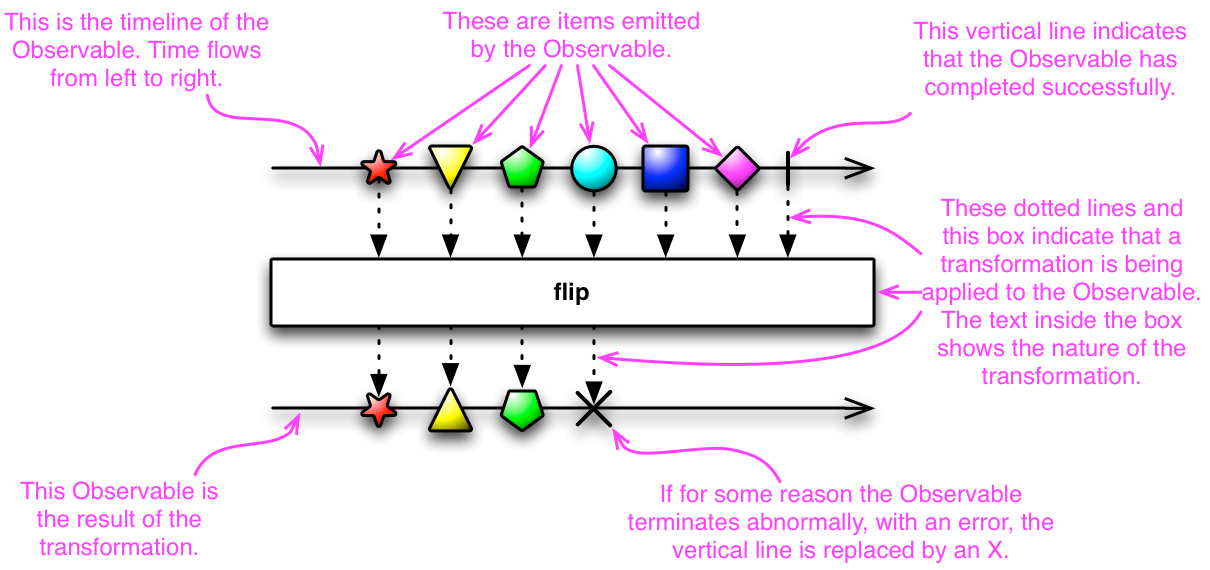
\includegraphics[width=0.9\textwidth]{img/Observable.png}
    \caption{Datenstrom Datenstrom orientierte Verarbeitung modelliert als Observable \cite[vgl. Abschnitt zu Observable]{rxAllgDoku} }
    \label{Observable}
  \end{centering}
\end{figure}
Kombiniert man die reaktive Programmierung mit Elementen der funktionalen Programmierung kann die Verarbeitung dieser Ströme elegant verkettet oder manipuliert werden. Die Kombination dieser Programmierparadigmen wird auch funktional-reaktive Programmierung genannt.
\newline
\newline
\newline
Bruce Eckel und Jonas Boner propagieren mit ihrem Reactive Manivesto den reaktiven Programmierstiel u.a. zusammen mit dem Bestreben nach \glqq Responsive Appliactions\grqq also ansprechbaren Applikationen, insbesondere GUI Applikationen, welche bei keiner Aktion blockieren dürfen \cite{heiseReactiveManifesto}. Dieses Manifest hebt die Bedeutung für aktuelle und zukünftige Applikationen hinsichtlich der Ansprechbarkeit seitens des Nutzerinterfaces hervor und soll Entwickler, sowie Softwarehersteller dazu aufrufen, das reaktive Paradigma zu evaluieren und im Idealfall gewinnbringend einzusetzen \cite{reactiveManifesto}.

\subsection{RX JAVA Entstehung}
RXJava ist eine Implementierung der Reactive Extensions (RX) für die Java Virtuelle Maschine. Reactive Extensions wurden von Erik Meijer erstmals für die .Net Plattform von Microsoft veröffentlicht mit dem Ziel, mittels funktional-reaktivier Programmierung die Verarbeitung von Event und Daten Strömen zu realisieren. In Meijers Konzept zu Reactive Extensions sind diese Ströme von Events oder Daten modelliert als sog. \glqq observierbare Ströme\grqq (eng. observable streams) (siehe hierzu auch das vorherige Kapitel 2.4.2). Die Ractive Extensions waren bislang nur für die funktionale Programmierung verfügbar. Die Firma Netflix hat es sich somit zur Aufgabe gemacht für ihren gleichnamigen Streaming Dienst eine eigene reaktive Erweiterung zur Java Standart Edition in der Version 7 mit dem RXJava heraus zu bringen. Die Entwicklung dieser Erweiterung hat das Ziel ein Framework für nicht blockierende (responsive) Applikationen, insbesondere für Gui Applikationen zur Verfügung zu stellen, welches dem Anspruch des Reactive Manifesto gerecht wird. Die Motivation den Streamingdienst mit der Entwicklung der reaktiven Erweiterung voranzutreiben liegt darin, ein Framework für die Entwicklung von nicht blokierenden NETFLIX Applikationen durch Drittanbieter zur Verfügung zu stellen. Dadurch dass, der Erfolg des Streaming Dienstes u.a. von der Akzeptanz der Applikation auf dem jeweiligen Endgerät (Playstation, XBOX, Android, IOS, Amazon TV, SmartTV) abhängig ist, hat Netflix zwangsläufig Interesse daran, dass die Implementierungen, die ständige Ansprechbarkeit durch den Nutzer gewährleisten und nicht blockieren. Aus diesem Grund hat Netflix seine reaktive Erweiterung auch für unterschiedliche Programmiersprachen veröffentlicht:
\begin{figure}[H]
  \begin{centering}
    
\includegraphics[width=0.9\textwidth]{img/rx-languages.png}
    \caption{(Netflix)RX kompatible Programmiersprachen}
    \label{rx-languages}
  \end{centering}
\end{figure} 
Die Reaktive Erweiterung für die JAVA SE von Netflix bietet also eine Chance für genau die, in dieser Arbeit diskutierte Problemstellung der Nebenläufigkeit unter Android. Der Quellcode zu RXJava kann als OpenSource Projekt im GitHub \texttt{ReactiveX/RxJava} bezogen werden. Auch die Einbindung in Softwareprojekte wird mittels diverser Dependency Management Tools unterstützt (Maven, Ivy, etc.). Wie die Reaktive Erweiterung konkret funktioniert wird zunächst an einem einfachen Implementierungsbeispiel für die Java SE vorgestellt und weiter auf das in den letzten Abschnitten diskutierte Beispiel unter Android transferiert.
\subsection{RXJava Funktionsweise}
Reactive Java oder RXJava stellt eine konkrete Implementierung des Beobachter Entwurfmusters der Reactive Extension dar. Darin wird beschreiben wie ein Objekt (Observable) bestimmte Elemente (Items) emittiert. Dabei kann sich ein weiteres Objekt (Observer oder Subscriber) für den Empfang der Items registrieren, womit dieses ab dem Zeitpunkt der Registrierung alle emittierten Items empfängt. Erweitert wird dies durch die Eigenschaft, nach der ein Observable die Registrierung von mehreren Subscribern zulässt und seine Items an diese emittiert. Die Bindung (Subscription) zwischen Observable und Subscriber kann jeder Zeit vom Subscriber widerrufen werden. Obsevables können gegenüber anderen Observables als Subscriber auftreten und von diesen weitere Items beziehen. Diese Items können daraufhin beliebig weiterverarbeitet werden (z.B. filtern, transformieren, gruppieren) und final für die registrierten Subscriber emittiert werden.\newline
Die Funktionsweise von RXJava wird im Folgenden an Hand eines einfachen Beispiels demonstriert und erläutert. In dem Beispiel wird ein einfaches Concurrency Szenario modelliert. Danach werden zwei Threads parallel gestartet. Diese sollen eine zeitaufwändige Operation, je zehn mal durchführen (Suchen einer großen Primzahl, siehe Kapitel 2.1).Die jeweiligen Ausgaben der Threads stellen den Datenstrom dar, der mittels der Observables und der Subscriber von RXJava verarbeitet wird. Die Ergebnisse der Verarbeitung werden auf der Konsole ausgegeben und sollen den Programmablauf zur Laufzeit wiederspielen. Der folgende Auszug zeigt den Sourcecode einer ersten Testanwendung. Die Klasse ReactiveDemo definiert ein Observable in dem eine zeitaufwändige Primzahlenoperation definiert ist. Dieser Code sollte analog zu den Beispielimplementierungen der vorangegangenen Kapitel nicht im Main Thread ablaufen, sondern in einem sekundären Hintergrundthread.\newline
\texttt{\newline
static Observable<String> myObservable = Observable.create(\newline
           new Observable.OnSubscribe<String>() \{\newline
               @Override\newline
               public void call(Subscriber<? super String> sub) \{\newline
                   for (int i = 0; i < 10; i++)\newline
      \{\newline
                       sub.onNext(\grqq ObserverThread: Hello, world!\grqq + i);\newline
                       BigInteger veryBig = new BigInteger(500, new Random());\newline
                       veryBig.nextProbablePrime();\newline
                   \}\newline
                   sub.onCompleted();\newline
               \}\newline
           \}\newline
   );\newline
}\newline
Das Observable stellt eine in sich geschlossene Verarbeitung einer Aufgabe dar. In diesem Fall werden dabei zehn Ergebnismengen durch folgenden Aufruf ermittelt:\newline\newline
\texttt{sub.onNext(ergebniss vom typ t)}\newline
\newline
Alle Subscriber, die sich zu diesem Observable registriert haben erhalten dann mittels der Rückrufmethode das Ergebnis in der \texttt{onNext()}-Methode. Ist die Verarbeitung im Observable beendet und werden keine weiteren Items mehr emittiert, so ruft das Observable die Rückrufmethode \texttt{onCompleted()} der bei ihm registrierten Subscriber auf. Analog wird im Fehlerfall verfahren und der Fehler an die einzelnen Subscriber übermittelt. Unser Beispiel definiert zwei Subscriber die jeweils zu einer eigenen Instanz des Observable registriert werden.\newline
\texttt{\newline
static Subscriber<String> myFirstSubscriber = new Subscriber<String>() \{\newline
\newline
       @Override\newline
       public void onNext(String s) \{\newline
           System.out.println("1rst Thread itemProcessing:");\newline
           System.out.println(s);\newline
       \}\newline
\newline
       @Override\newline
       public void onCompleted() \{\newline
           firstObservableHasFinished=true;\newline
           System.out.println("1rst item Completed");\newline
       \}\newline
\newline
       @Override\newline
       public void onError(Throwable e) \{\newline
           System.out.println("There was an error on first subscriber:" + e);\newline
       \}\newline
   \};\newline
\newline
   static Subscriber<String> mySndSubscriber = new Subscriber<String>() \{\newline
       @Override\newline
       public void onNext(String s) \{\newline
           System.out.println("  2ndThread: itemProcessing:");\newline
           System.out.println(s);\newline
       \}\newline
\newline
       @Override\newline
       public void onCompleted() \{\newline
           secondObservableHasFinished = true;\newline
           System.out.println("2nd Thred: item Completed");\newline
       \}\newline
\newline
       @Override\newline
       public void onError(Throwable e) \{\newline
       \}\newline
   \};\newline
}
Die Subscriber implementieren folgende Rückruf Methoden für den Aufruf durch Observables:
\begin{itemize}
\item \texttt{onNext()}
\item \texttt{onComplete()}
\item \texttt{onError()}
\end{itemize}
Dabei handelt es sich um vom Framework vorgegebene Standart Rückruf Methoden, die je nach Subscription von unterschiedlichen Observables angesprochen werden können. Die Subscription selbst enthält darüber hinaus noch zusätzliche Konfigurationen. So ist genau definiert, dass die Observierung durch die Subscriber selbst in dem MainThread laufen sollen (\texttt{.observeOn(Schedulers.io())}) und die Verarbeitung des Observables in einem sekundären Thread stattfindet (\texttt{subscribeOn(Schedulers.newThread())}). Das bedeutet, dass das Observabel auf zwei Threads dubliziert wird, für jeweils den Subscriber eins und 
Subscriber zwei. Dagegen laufen beide Subscriber Instanzen auf dem Main Thread.\newline
\texttt{\newline
Subscription subscriptionOne =\newline myFirstObservable.subscribeOn(Schedulers.newThread())
\newline.observeOn(Schedulers.io()).subscribe(myFirstSubscriber);\newline
\newline
Subscription subscriptionTwo =\newline mySecondObservable.subscribeOn(Schedulers.newThread())
\newline.subscribe(mySecondSubscriber);\newline
}\newline
Bei dieser Beispiel Anwendung handelt es sich um eine einfache Java Applikation, die durch die \texttt{main()}- Methode gestartet und darin die angesprochene Verarbeitung innerhalb eines Observables in zwei sekundären Threads auslagert. Wird diese Applikation nun gestartet, so würde sie wieder terminieren, bevor die Verarbeitung in den sekundär Threads abgeschlossen ist. Dem entsprechend wird eine fortwährende Verarbeitung im Main Thread durch eine \texttt{while}- Schleife simuliert, deren Abbruchkriterium der Status Completed der Observables von beiden Sekundär Threads ist. Das Ergebnis ist Folgendes (siehe nächste Seite):\newpage


\begin{table}[h!]
  \begin{center}
    \label{tab:table2}
    \begin{tabular}{cc}
\midrule

1rst Thread itemProcessing:&  \\
ObserverThread: Hello, world!0&  \\
              	  					&  2ndThread: itemProcessing:\\
             						 &  ObserverThread: Hello, world!0\\
1rst Thread itemProcessing:&  \\
ObserverThread: Hello, world!1&  \\
1rst Thread itemProcessing:&  \\
ObserverThread: Hello, world!2&  \\
                               		& 2ndThread: itemProcessing:\\
                              		& ObserverThread: Hello, world!1\\
1rst Thread itemProcessing:&  \\
ObserverThread: Hello, world!3&  \\
1rst Thread itemProcessing:&  \\
ObserverThread: Hello, world!4&  \\
                            		& 2ndThread: itemProcessing:\\
                               		& ObserverThread: Hello, world!2\\
1rst Thread itemProcessing:&  \\
ObserverThread: Hello, world!5&  \\
                          	   		& 2ndThread: itemProcessing:\\
                               		& ObserverThread: Hello, world!3\\
                               		& 2ndThread: itemProcessing:\\
                               		& ObserverThread: Hello, world!4\\
                               		& 2ndThread: itemProcessing:\\
                               		& ObserverThread: Hello, world!5\\
                               		& 2ndThread: itemProcessing:\\
                               		& ObserverThread: Hello, world!6\\
1rst Thread itemProcessing:&  \\
ObserverThread: Hello, world!6&  \\
                               		& 2ndThread: itemProcessing:\\
                               		& ObserverThread: Hello, world!7\\
1rst Thread itemProcessing:&  \\
ObserverThread: Hello, world!7&  \\
                               		& 2ndThread: itemProcessing:\\
                               		& ObserverThread: Hello, world!8\\
1rst Thread itemProcessing:&  \\
ObserverThread: Hello, world!8&  \\
                               		& 2ndThread: itemProcessing:\\
                               		& ObserverThread: Hello, world!9\\
                               		& 2nd Thred: item Completed\\
1rst Thread itemProcessing:&  \\
ObserverThread: Hello, world!9&  \\
1rst item Completed&  \\
\bottomrule
    \end{tabular}
  \end{center}
\end{table}
\newpage
Zusehen ist hier wie in unterschiedlichen Threads die Observables abwechselnd ihre Iterationen 0-9 durcharbeiten, die Ergebnismengen an den jeweiligen Subscriber im Main Thread schicken und dieser die Ausgaben auf der Konsole ausgibt.  
Die erste Beispielimplementierung zu RXJava zeigt wie asynchrone Verarbeitung in sekundäre Threads ausgelagert werden kann und dabei die Ergebnisübergabe mittels Rückrufmethoden realisiert ist. Diese sind fest vordefiniert im Main Thread und werden reaktiv erst dann angesteuert, wenn von dem registrierten Observable ein Ereignis vorliegt. Zu den Ereignissen gehören entsprechend der Rückrufmethoden:
\begin{itemize}
\item Es liegt eine neue Ergebnismenge vor $\rightarrow$ \texttt{onNext()}
\item Es liegt ein Fehler bei der Verarbeitung innerhalb des Observables vor $\rightarrow$ \texttt{onError()}
\item Die Verarbeitung im Observable ist abgeschlossen $\rightarrow$ \texttt{onNext()}
\end{itemize}
Die Dokumentation zu RXJava zeigt zu oben genanntem Beispiel, wie Observables miteinander verkettet werden können und somit unterschiedliche Verarbeitungsketten realisierbar sind:
ObserverWorkerChain
\begin{figure}[H]
  \begin{centering}
    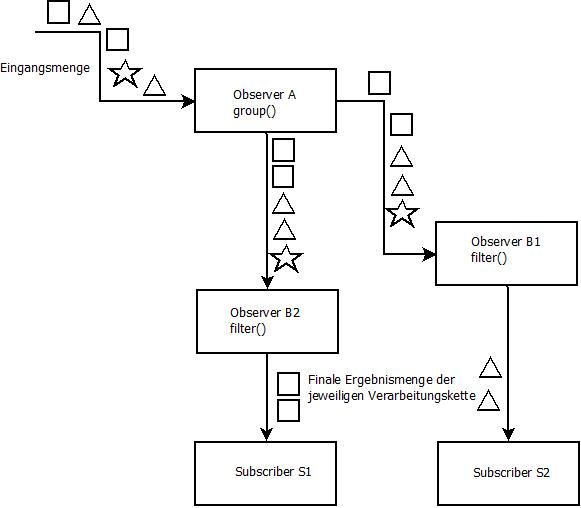
\includegraphics[width=0.9\textwidth]{img/ObserverWorkerChain.jpeg}
    \caption{Komplexe Verarbeitungskette mit mehreren Observern}
    \label{ObserverWorkerChain}
  \end{centering}
\end{figure}
In o.g. Abbildung tritt ein Observable selbst als Subscriber auf und erwartet von dem Observable zu dem er sich registriert hat seine Eingangswerte die er seinerseits weiterverarbeitet. Die Ergebnismenge stellt dieses Observable dann wieder seinen Subscribern zur Verfügung usw. RXJava bietet an dieser Stelle noch praktische vordefinierte Observables die nach Bedarf genutzt werden können und den Sourcecode vereinfachen. In o.g. Graphik dienen die vordefinierten Observables dazu zunächst die Eingangsdaten zu gruppieren (siehe Observable A group()) und weiter die gruppierten Daten zu filtern (siehe Observable B1 und B2 filter()). Zu dem Empfang der Ergebnismengen der Verarbeitungsketten registrieren sich abschließend die Subscriber S1und S2.

\subsection{RXJava in Android}
Der letzte Abschnitt hat gezeigt wie mittels RXJava im Vergleich zu den Mitteln aus der Java SE relativ leicht asynchrone Verarbeitung realisiert werden kann. Doch nun gilt es dies auch für Android Applikationen zu realisieren. Für den Einsatz von RXJava gibt es eine sinnvolle Erweiterung, welche die Entwicklung erleichtert. RXAndroid ist ein Packet, welches einfach in die Android Applikation eingebunden werden kann. Das Packet erleichtert besonders mit vordefinierten Scheduler die Entwicklung. Soll die Verarbeitung des Observables oder des Subscribers auf dem Android Main Thread laufen, so bietet die RXAndroid Erweiterung den AndroidScheduler an. Für das in dieser Arbeit betrachtete Szenario zur Nebenläufigkeit (siehe Kapitel 1.5) würde es dementsprechend Sinn machen, die zeitintensive Verarbeitung im Observable als Sekundär Thread auszulagern (\texttt{.subscribeOn(Schedulers.newThread())}) und den Subscriber, der asynchron die Ergebnismenge des Observables erhält, im Main Thread der Android Anwendung laufen zu lassen (\texttt{observeOn(AndroidSchedulers.mainThread())}). Demnach wird für unsere Beispielimplementierung die Subscription wie folgt in der Activity der Applikation definiert:\newline
\texttt{\newline
private Subscription getSubscription(Subscriber<String> aSubscriber) \{\newline
       RandomPrimeNumGenerator randomPrimeNumGenerator =\newline 
       new RandomPrimeNumGenerator();\newline
\newline
       return randomPrimeNumGenerator.getObservable().\newline
       observeOn(AndroidSchedulers.mainThread())\newline
               .subscribeOn(Schedulers.newThread())\newline
               .subscribe(aSubscriber);\newline
   \}\newline
   }\newline
Der o.g. Codeauszug zeigt eine Methode der Activity unserer Beispielimplementierung, die zu einem gegebenen Subscriberobjekt eine Subscribtion erstellt. Hierzu wird eine Instanz vom Typ \texttt{RandomPrimeNumGenerator} erzeugt die ein Observable zurückliefert und zu dem ein gegebener Subscriber registriert wird. Die im Szenario geforderte zeitintensive Verarbeitung ist durch das Observable gekapselt. Der folgende Quellcode zeigt hierzu einen Auszug aus der Klasse \texttt{RandomPrimeNumGenerator}, die dieses Observable implementiert:\newline
   \texttt{\newline
 public RandomPrimeNumGenerator()\newline
   \{\newline
   primMessageObservable = Observable.create(\newline
           new Observable.OnSubscribe<String>() \{\newline
               @Override\newline
               public void call(Subscriber<? super String> sub) \{\newline
               \newline
                   for(int i=0; i<10; i++)\newline
                   \{\newline
                       BigInteger veryBig = new BigInteger(500, new Random());\newline
                       BigInteger randomPrimeNumber = veryBig.nextProbablePrime();\newline
                       int summe = 0;\newline
                       while (0 != randomPrimeNumber.compareTo(BigInteger.ZERO)) \{\newline
                           // addiere die letzte ziffer der uebergebenen zahl zur summe\newline
                           summe = summe + (randomPrimeNumber.mod(BigInteger.TEN)).intValue();\newline
                           // entferne die letzte ziffer der uebergebenen zahl\newline
                           randomPrimeNumber = randomPrimeNumber.divide(BigInteger.TEN);\newline
                       \}\newline
\newline
                      sub.onNext("Observable emits CrossSum for iteration: " + i );\newline
                      sub.onNext(String.valueOf(summe));\newline
                  \}\newline
                   sub.onCompleted();\newline
              \}\newline
           \}\newline
   );\newline
\newline
  public Observable<String> getObservable()\{\newline
       return primMessageObservable.filter(new Func1<String, Boolean>() \{\newline
                   @Override\newline
                   public Boolean call(String item) \{\newline
                       try \{\newline
                           Integer.valueOf(item);\newline
                       \} catch (NumberFormatException e) \{\newline
                           return false;\newline
                       \}\newline
                       return true;\newline
               \}\}\newline
               );\newline
   \}\newline
}\newline
Das Observable emittiert also hier pro Iteration zwei Items. Zum Einen den String zur Identifikation der Iteration:\newline
\texttt{\newline
sub.onNext(\grqq Observable emits CrossSum for iteration: \grqq + i );\newline
}\newline
zum Anderen die berechnete Primzahl selbst:\newline
\texttt{\newline
sub.onNext(sub.onNext(String.valueOf(summe));\newline
}\newline
Der o.g. Quellcodeauszug der Activity zeigt in seiner \texttt{getObservable()} Methode, wie mittels eines Filter Observables nur das Ergebnis (hier der Integerwert) zum Subscriber weitergeleitet wird. Entspechend registriert sich der Subscriber beim Filter Observable. Die Activity definiert zwei Subscriber, die unterschiedlich aus der Gui angestoßen werden können.\newline
\texttt{\newline
private Subscriber<String> getFirstSubscriber() \{\newline
\newline
       return new Subscriber<String>() \{\newline
           @Override\newline
           public void onNext(String s) \{\newline
               //Actualize the view + setting value\newline
               String lastOutput = firstObserverOutput.getText().toString();\newline
               firstObserverOutput.setText(lastOutput + s);\newline
\newline
               firstObserverOutput.invalidate();\newline
           \}\newline
\newline
           @Override\newline
           public void onCompleted() \{\newline
               //show in view that observer is ready\newline
           \}\newline
\newline
           @Override\newline
           public void onError(Throwable e) \{\newline
               //show in view that observer ran in an error\newline
           \}\newline
       \};\newline
   \}\newline
\newline
   private Subscriber<String> getSecondSubscriber() \{\newline
\newline
       return new Subscriber<String>() \{\newline
           @Override\newline
           public void onNext(String s) \{\newline
               //Actualize the view + setting value\newline
               String lastOutput = secondObserverOutput.getText().toString();\newline
               secondObserverOutput.setText(lastOutput + s);\newline
\newline
               secondObserverOutput.invalidate();\newline
           \}\newline
\newline
           @Override\newline
           public void onCompleted() \{\newline
               //show in view that observer is ready\newline
           \}\newline
\newline
           @Override\newline
           public void onError(Throwable e) \{\newline
               //show in view that observer ran in an error\newline
           \}\newline
       \};\newline
   \}\newline
   }\newline
Je nach dem über welche ViewId die Initialisierung der Subscriber gestartet wird, ist zu entschieden, welche Subscriber Implementierung zu verwenden ist um eine Subscribtion zu starten.\newline
\texttt{\newline
 public void initSubscription(View aView) \{\newline
       if (aView.getId() == R.id.startSubscription1) \{\newline
           firstSubscriber = getFirstSubscriber();\newline
           subscription1 = getSubscription(firstSubscriber);\newline
\newline
       \}\newline
       if (aView.getId() == R.id.startSubscription2) \{\newline
           secondSubscriber = getSecondSubscriber();\newline
\newline
           subscription2 = getSubscription(secondSubscriber);\newline
       \}\newline
   \}\newline
}\newline
Die jeweilige Referenz einer Subscribtion wird in einer Klassenvariable der Activity gespeichert, um diese im Falle einer ungeplanten Terminierung der Activity-Instanz vorher noch zu beenden. Dies gilt z.B. für das Event \grqq Configuration Change\grqq nachdem standardgemäß die aktuelle Activity-Instanz zerstört und neu erstellt wird (siehe hierzu auch Kapitel 1.4 den Lebenszyklus einer Activity). Der folgende Codeauszug zeigt, wie der Aufruf \texttt{unsubscribe()} für die jeweilige Subscribtion genau das leistet. Der Empfang der Items wird abgebrochen noch bevor das Observable den Status \grqq Completed\grqq erreicht hat.\newline
\texttt{\newline
@Override\newline
   public void onDestroy() \{\newline
       if (subscription1 != null) \{\newline
           subscription1.unsubscribe();\newline
       \}\newline
       if (subscription2 != null) \{\newline
           subscription2.unsubscribe();\newline
       \}\newline
   \}\newline
}

\section{Zusammenfassung}
In diesem Kapitel werden drei unterschiedliche Konzepte zur Realisierung von Nebenläufigkeit in Bezug auf das Android Betriebssytem vorgestellt. Um diese Konzepte vergleichbar zu machen ist ein Beispiel Szenario definiert, indem eine oder mehrere zeitaufwändige Operationen innerhalb einer Android Applikation gestartet werden. In einer ersten Beispiel Implementierung ohne jegliche Nebenläufigkeit haben wird deutlich, wie durch Starten einer zeitaufwändigen Operation die Anwendung nicht mehr auf Benutzereingaben reagiert. Je nach Wartedauer meldet sich dabei nach kurzer Zeit die Applikation mit dem Ergebnis der Operation zurück oder nach längerer Wartezeit erscheint der Application Not Responding Dialog. Dieser gibt dem Nutzer die Möglichkeit entweder weiter auf die Rückmeldung der Anwendung zu warten, oder die Anwendung abzubrechen. Um zu Untersuchen wie die jeweiligen Konzepte die Ansprechbarkeit der Anwendung gewährleisten und gleichzeig die zeitaufwändige Operation im Hintergrund durchführen, werden in den letzten Abschnitten entsprechende Beispielimplementierungen  vorgestellt.\newline
In der ersten Implementierung wird mittels der Funktionalitäten aus der Java Standard Edition versucht, die zeitaufwändige Operation in eine Hintergrundverarbeitung (sekundär Thread) auszulagern. Um den Nachrichtenaustasch zwischen dem sekundär Thread und dem Main Thread (verantwortlich für Verarbeitung der Benutzerinteraktion) der Anwendung zu realisieren wird ein spezieller Mechnismus vorgestellt und angewandt. Dabei handelt es sich um den Handler Looper Mechanismus aus dem Android SDK. Dieser Mechanismus bietet sich dadurch an, dass er standardgemäß durch das Betriebssystem für jede Anwendung initialisiert wird, um den applikationsinternen Nachrichtenaustausch zwischen unterschiedlichen Komponenten der Anwendung zu realisieren.\newline
Im Kapitel 2.3 wird ein Konzept aus dem Android SDK selbst vorgestellt, mit dem nebenläufige Verarbeitung realisierbar ist. Mit der Android AsyncTask Funktionalität wird die Kapselung, Initialisierung und Auswertung (Erfolg oder Fehlerbehanldung) von nebenläufiger Verarbeitung in klar definierte abstrakte Methoden unterteilt. Die darin definierte Logik wird entsprechend durch den AsyncTask auf Sekundär- und Main- Thread verteilt. Der Nachrichtenaustauch zwischen den Threads ist dabei auch hier durch den Handler Looper Mechanismus realisiert. Der Fokus dieses Konzeptes liegt auf der möglichst einfachen Realisierung von Hintergrundverarbeitung durch den Entwickler. Dabei wird jedoch in der Standartvariante lediglich ein Hintergrund Thread erzeugt. D.h. im Falle von mehreren zeitaufwändigen Operationen werden diese seriell in einem Hintergrund Thread abgearbeitet, was mit unter sehr zeitintensiv und unperformant im Hinblick auf weitere Parallelisierungen besonders im Multicore-Betrieb sein kann. \newline
Das dritte Konzept zur Nebenläufigkeit unter Android versucht die Hintergrundverarbeitung mittels reaktiver Programmierung zu realisieren. Dabei fließen Eingenschaften der funktionalen Programmierung in die eher prozedurale Programmierung von Android Applikationen mittels Java ein. Das Framework RXJava abstrahiert dabei von der Thread -Erzeugung, sowie über die Inter- Thread Kommunikation mittels standartisierter Rückrufmethoden. Der funktionale Ansatz führt zu einer Datenstrom orientierten Verarbeitung, in der die einzelnen Verarbeitungsschritte insich geschlossene Funktionen darstellen. Innerhalb der Verarbeitungskette werden die Funktionen als Returnwert einer Operation übergeben, um sie in Abhängigkeit der eintreffenden Daten im jeweiligen Kontext auszuführen.  Die Verarbeitungsketten werden mittels der Rückrufmethoden dann angesteuert, wenn ein Ergebnis aus der Hintergrundverarbeitung vorliegt. Dies können Zwischenergebnisse oder Status / bzw. Fehlermeldungen sein.
Die Hintergrundverarbeitung in Sekundär- Threads wird mittels einfacher vordefinierter Scheduler definiert. Der Entwickler muss sich dabei weder um die korrekte Erzeugung noch um die Synchronisation beim Nachrichtenaustausch zwischen sekundär und Main Thread kümmern. \newline

\chapter{Konzepte der Nebenläufigkeit im kritischen Diskurs}
In diesem Kapitel steht der kritische Vergleich der im letzten Kapitel vorgestellten Konzepte der Nebenläufigkeit unter Android im Vordergrund. Dabei werden Chancen und Risiken der einzelnen Konzepte beleuchtet mit dem Ziel, daraus eine Erkenntnis abzuleiten, für welche Implementierungszenarien sich ein Konzept womöglich mehr oder weniger eignen könnte.

\section{Chancen und Risiken des Java Concurrency Konzepts}
Das Implementierungsbeispiel hat gezeigt wie mittels der Werkzeuge aus der Java Standard Edition auf elementarer Ebene Nebenläufigkeit konzipiert werden kann. Erfahrene Entwickler, die sich mit Multi Threading auskennen, erhalten besonders mit dem neuen Concurrency Packet von Java 7 zahlreiche Möglichkeiten um Hintergrundverarbeitung exakt nach ihren Anforderungen erstellen zu können. Der Entwickler kann damit auf sehr feingranularer Ebene die Steuerung der Hintergrundverarbeitung anpassen. Die dafür verwendeten Werkezuge, werden unter dem allgemeinen Java Standart gepflegt, was für einen langfristigen Einsatz eine gewisse Sicherheit in Bezug auf die Zukunftsträchtigkeit der Werkzeuge mitsich bringt. Die Konzeption von allgemeiner Nebenläufigkeit mittels der Standartwerkzeuge findet breite Anwendung und ist daher in zahlreicher Fachliteratur erläutert. Die Standartwerke hierzu sind Java Concurrency und Java Concurrency in Practice.  Zusätzlich sind ausreichend freie Tutorials im Internet verfügbar. Die Nebenläufigkeit mit Java SE Werkzeugen unter Android und die damit verbundenen Besonderheiten, sind dagegen deutlich schlechter dokumentiert. So ist es ratsam sich das Wissen über die Lebenszyklen, den Botschaftenaustausch, etc. in Android spezifischen Literaturquellen an zu eignen.
Im Hinblick auf eine langfristige Wartung der Applikationen ist es durch aus von Vorteil dass diese Form der Nebenläufigkeit auf Standartbibliotheken basiert. Dadurch, dass das aktuelle Android SDK auf der Java Standard Edition in der Version 7 aufsetzt, verfügt der Entwickler bereits über alle benötigten Werkzeuge und er muss keine zusätzlichen Bibliotheken einbinden.
Eine doch schon bei der Entwicklung des Prototypen zur Hintergrundverarbeitung aufgetretene Schwierigkeit ist die hohe Komplexität, die Fehleranfälligkeit und das Problem der schlechten Übersichtlichkeit im Code bei mehreren Hintergrundverarbeitungen. Dies birgt ein nicht zu unterschätzendes Fehlerpotential. In Kapitel 1.2.3 wird bereits auf die allgemeinen Risiken der Nebenläufigkeit eingegangen. Bei fehlerhafter Implementierung ist hier die Gefahr von Speicherlecks besonders präsent, denn um diese zu verhindern muss der Entwickler über entsprechendes Spezialwissen verfügen, insbesondere zu der korrekten Referenzierung/bzw. Dereferenzierung von Objekten innerhalb der Activity einer Anwendung (siehe Kapitel 2.2.3).
\section{Android Concurrency}
Um dem Problem der Nebenläufigkeit zu begegnen liefert Google in seinem Android SDK mit der Klasse android.os.AsyncTask eine auf Android spezialisierte Lösung. Diese charakterisiert sich im wesentlichen dadurch, dass sie von der Definition der Nebenläufigkeit auf Threadebene abstrahiert und dem Entwickler vordefinierte Methoden für die Hintergrundberechnung, die Fehlerbehandlung, sowie die Ergebnisübergabe anbietet. Android AsyncTak ist auf die Besonderheiten von Android wie z.B. den applikationsinternen Botschaftenaustausch zugeschnitten. Dabei wird ebenfalls der Handler Looper Mechanismus verwendet. Der höhere Grad der Abstraktion im Vergleich zum JavaConcurrency Konzept ermöglicht es dem Entwickler eine einfache Hintergrundberechnung zu definieren, ohne sich um Thread -Erzeugung, -Synchronisation, oder dem Botschaftenaustausch zu kümmern. Dabei rät die Android Developper Dokumentation diese Lösung explizit nur für kurze Hintergrundoperationen zu verwenden. Dadurch, dass Android AsyncTask lediglich einen Hintergrundgrund Thread in der Standart Konfiguration verwendet, wird diese Lösung für mehrere aufwändige Operationen unperformant, da die Verarbeitung entsprechend serialisiert werden müssten. Alternativ wird hier auch das Multi Threading unterstützt. Die Dokumentation zu Android AsyncTask ist für die Standart Konfiguration (nur ein Hintergrund Thread wird gestarted) detailliert und mit übersichtlichen Beispielimplementierungen versehen und lässt damit einen  schnellen Einstieg in diese Technologie zu. Ein Entwickler benötigt hierzu fast keine Kenntnisse über das Multi Threading in Java. Dagegen ist die Konfiguration für mehrere Hintergrund Threads nicht ausreichend dokumentiert. Es wird lediglich davor gewarnt, mehrere Hintergrund Threads zu verwenden, da es hierbei zu unerwarteten Seiteneffekten, sowie Reihenfolgeproblemen kommen kann. Entsprechend bleiben Fragen u.a. zu dem konkreten Ablauf der Hintergrundverarbeitung mit mehreren Threads unbeantwortet und müssen aus der Implementierung von AsyncTask und der verwendeten Scheduler hergeleitet werden (siehe hierzu Kapitel 2.x).\newline
Ein weiterer Punkt ist die problematische Steuerung der Nebenläufigkeit nachdem diese initialisiert wurde. Zwar lässt sich jederzeit der Status der Verarbeitung an den Main Thread übertragen, jedoch lässt sich diese z.B. nicht aus dem Main Thread heraus beenden, da die Inter-Thread Kommunikation auf den unidirektionalen Nachrichtenweg beschränkt ist und weitere Steuerungsmechanismen nicht vorgesehen sind. Dies kann durchaus zu einem Problem werden, wenn die Applikation pausiert oder beendet wird. In diesem Fall kann es passieren, dass eine angestoßene Hintergrundverarbeitung weiterläuft und unnötig Ressourcen verbraucht.\newline
Abschließend ist zu nennen, dass Google diese Lösung mit dem Standard SDK bereitstellt und für die Konzeption von Nebenläufigkeit keine zusätzlichen Bibliotheken benötigt werden.

\section{RXConcurrency}
Die Beispielimplementierung aus Kapitel 2.xx hat gezeigt, wie bei der Nutzung von RXJava ein Paradigmenwechsel von der prozeduralen Programmierung hin zu einem eher funktionalen Programmierstiel vom Entwickler zu leisten ist. Dabei wird die Nebenläufigkeit auf einem hohen Abstraktionsniveau definiert, wodurch die Entwicklung selbst einfacher und weniger Fehleranfällig wird. Dabei stellt u.U. der Wechsel hin zur funktionalen Programmierung für Entwickler die bislang primär prozedural entwickelten eine hohe Einstiegshürde dar. Die Dokumentation von RXJava liefert jedoch ausreichend Material um den Wechsel zur hier verwendeten reaktiv-funktionalen Programmierung zu leisten, sowie um damit stabile Hintergrundberechnungen zu konzipieren. Dabei unterstützt das Framework den Entwickler durch vorgegebene Methoden zur Ergebnisübergabe, sowie der Status- und Fehlermeldung an den Main Thread. Zusätzlich bietet RXJava eine Steuerungsmöglichkeit um eine laufende Hintergrundberechnung zu terminieren (siehe unSubscribe()-Mechanismus in Kapitel 2.xxx). Diese Steuerungsmöglichkeit ist einfach in eine Android Applikation zu integrieren und bietet sich in Bezug auf den Lebenszyklus der Applikation an, um Speicherlecks zu vermeiden. Die nebenläufige Verarbeitung kann mittels RXJava auf beliebig viele Threads verteilt werden. Einzige Vorraussetzung dafür ist, zu jedem Thread ein Observable zu definieren. Dabei ist der Quellcode durch den funktionalen Programmierstiel übersichtlich und auf das Wesentliche, nämlich die Verarbeitung, konzentriert.\newline
Ein potentielles Risiko birgt die Tatsache, dass RXJava zwar durch ein namhaftes Unternehmen (Netflix) entwickelt und vorangetrieben wird, die Bibliothek als solche aber keinen Standard darstellt, oder in einer Standardbibliothek integriert ist. Dadurch besteht für eine langfristige Wartung von Applikation, die über Abhängigkeiten zu RXJava verfügen die Gefahr, dass RXJava eines Tages nicht mehr weiter gepflegt wird. Daraus können im schlimmsten Fall große Refaktorisierungsaufwände entstehen.


\section{Szenariobasierte Analyse}
Die in dieser Arbeit vorgestellten Konzepte der Nebenläufigkeit in Bezug auf Applikationen unter dem Android Betriebssystem beinhalten unterschiedliche Chancen und Risiken in Bezug auf den jeweiligen Praxiseinsatz. Dieser Abschnitt versucht die vorgestellten Konzepte mit unterschiedlichen Szenarien in Beziehung zu setzen, um daraus Aussagen für konkrete Praxiseinsätze ableiten zu können.\newline
Die folgende Graphik betrachtet die in dieser Arbeit diskutierten Konzepte der Nebenläufigkeit in Bezug auf unterschiedliche Szenarien. Dabei soll eine Auswahl von möglichst prägnanten Eigenschaften die Unterschiede in Abhängigkeit zum Einsatzkontext der Konzepte auf einen Blick deutlich machen. Hierzu wird die Ausprägung der jeweiligen Eigenschaft durch die Größe der Kreise symbolisiert. Es gilt demnach für die Eigenschaften:\newline \newline
\glqq Höhe der Einstiegshürde in Bezug auf den Wissensaufbau\grqq $\rightarrow$ je größer der Kreis, desto höher ist die Einstiegshürde \newline \newline
\glqq wie hilfreich ist die Dokumentation\grqq $\rightarrow$ je größer der Kreis, desto hilfreicher ist die Dokumentation\newline \newline
\glqq wie hilfreich ist der Abstraktionsgrad\grqq $\rightarrow$ je größer der Kreis, desto hilfreicher ist der Abstraktionsgrad\newline \newline
\glqq Gefahr von Fehlern bei der Implementierung\grqq $\rightarrow$ je größer der Kreis desto größer die Gefahr von Fehlern bei der Implementierung

\begin{figure}[H]
  \begin{centering}
    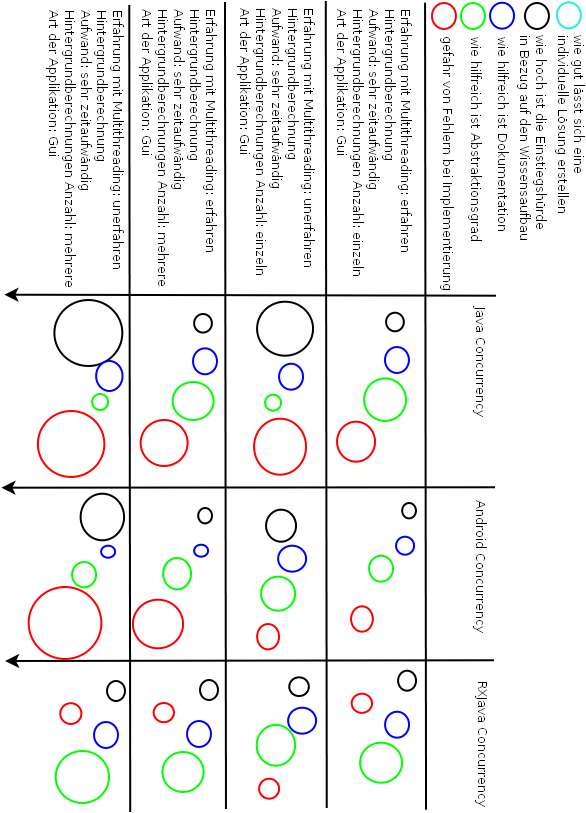
\includegraphics[width=1\textwidth]{img/szenarioBasedAnalysis.png}
    \caption{Vergleichsmatrix zur szenarienbasierten Analyse}
    \label{szenarioBasedAnalysis}
  \end{centering}
\end{figure}
\newpage
\paragraph{Szenario A:}
Das erste Szenario beschreibt einen Fall indem eine einzelne zeitaufwändige Hintergrundoperationen durch einen erfahrenen Entwickler zu konzipieren ist. Für einen Entwickler mit einem gewissen Erfahrungsschatz im Bereich der Nebenläufigkeit fallen zwei hervorstechende Merkmale in Bezug auf Java Concurrency auf. Zum einen kommt der in diesem Fall niedrige Abstraktionsgrad dem erfahrenden Entwickler entgegen, um das Konzept der Nebenläufigkeit möglichst exakt an seine Anforderungen und Vorstellungen auszurichten. Zum andern bietet aber auch genau dieser Abstraktionsgrad ein relativ hohes Fehlerpotential.
Das Konzept der Android Concurrency bietet dem erfahrenen Entwickler dagegen eher wenig individuelle Anpassungsmöglichkeiten jedoch ist es dafür auch deutlich weniger Fehleranfällig. Gegenüber der fehlenden individuellen Anpassungsmöglichkeiten steigt jedoch damit der Komfort bei der Entwicklung, denn durch den höheren Abstraktionsgrad wird der Code übersichtlicher und damit leichte wartbar.
Das Konzept der RXJava Concurrency bietet den höchsten Abstraktionsgrad und damit den meisten Komfort bei Konzeption und Wartung von Nebenläufigkeit, bei gleichzeitiger geringer Fehleranfälligkeit.
Für den erfahrenen Entwickler ist es damit eine Frage des Bedürfnisses nach maximaler Anpassbarkeit gegenüber maximalem Komfort.

\paragraph{Szenario B:}
Das nächste Szenario beschreibt die selben Anforderungen an Komplexität der Hintergrundberechnung, sowie deren Anzahl, wie Senario A. Der Unterschied liegt jedoch nun darin, dass ein eher ungeübter Entwickler die Konzeption von Nebenläufigkeit verantworten muss. Nun gewinnt der Punkt der Einstiegshürden in die jeweiligen Konzepte an Bedeutung. Entsprechend stellt die Java Concurrency eine hohe Einstiegshürde in Bezug auf den benötigten Wissensaufbau dar. Gleichermaßen ist durch die niedrige Abstraktionsebene in Zusammenhang mit fehlendem Wissen im Bereich des Multithreading, das Fehlerpotential in Relation zum Szenario A deutlich höher.
Die Android Concurrency verringert dagegen das Fehlerpotential bietet eine niedrige Einstiegshürde durch den höheren Abstraktionsgrad, sowie eine für dieses Szenario sehr passende und detaillierte Dokumentation.
Je nach Erfahrung mit der funktionalen Programmierung kann in diesem Szenario das Fehlerpotential durch die hohe Abstraktionsebene von RXJava weiter gesenkt werden. Zusätzlich bietet RXJava einfache Mechanismen zur Steuerung der Hintergrundverarbeitung. Dieser Punkt wird in der Android Concurrency eher vernachlässigt.
Für einen ungeübten Entwickler ist es u.U. ratsam genau zu verifizieren mit welchem Konzept zur Nebenläufigkeit unter Android er in absehbarer Zeit zu seinem gewünschten Ergebnis gelangt und welches Fehlerpotential damit einhergehen kann. Die Android Concurreny ist zwar genau darauf ausgelegt, eine einfache Hintergrundberechnung zu erzeugen, jedoch warnt die Dokumentation davor zu zeitaufwändige Berechnungen hiermit abzubilden, denn in diesem Fall besteht das Risiko von Memory Leaks, wenn die Hintergrundberechnung nicht zu bestimmten Zeitpunkten abgebrochen werden kann (siehe Kapitel 2.2.X).

\paragraph{Szenario C:}
In diesem Szenario steht wieder der erfahrene Entwickler im Fokus vergleichbar zum Szenario A. Nun jedoch sollen mehrere zeitintensive Hintergrundverarbeitungen parallel gestartet werden können. Dabei gibt es bei dem Java Concurrency keine nennenswerten Unterschiede in der Ausprägung der Merkmale zu Szenario A. Das liegt an dem niedrigen Abstraktionsniveau, welches dem Entwickler alle Möglichkeiten an die Hand gibt, eine individuelle Lösung gemäß der hier definierten Anforderungen zu erstellen. Lediglich das Fehlerpotential steigt bei diesem Szenario, da für mehrere parallele Hintergrundverarbeitungen evtl. die Thread Synchronisation und Steuerung zu Problemen führen könnte. Diese Fragestellungen fallen im Szenario A eher weniger ins Gewicht, da hier nur eine Hintergrundverarbeitung benötigt wird.
Das Konzept der Android Concurrency weist deutlichere Unterschiede auf zum Szenario A auf. Dadurch dass zu diesem Konzept die Dokumentation von der Erstellung mehrerer paralleler Hintergrundverarbeitungen (in mehreren parallelen Threads) abgeraten wird und dies auch nicht weiter dokumentiert wird, steigt deutlich das Fehlerpotential. Auch eignet sich die Abstraktionsebene weniger für diese Form der Hintergrundverarbeitung, da der Entwickler nur geringen Einfluss auf die Thread- Synchronisation, sowie deren Steuerung hat.
Das Konzept der RXJava Concurrency vereinfacht die hier geforderte Form der parallelen Hintergrundverarbeitung für den Entwickler. Dies geht jedoch zu Lasten der Anpassbarkeit, die hier nicht im Detail möglich ist, wie bei der Java Concurrency. Das Fehlerpotential ist dagegen vergleichsweise zu den anderen beiden Konzepten in diesem Szenario gering. Die etwas im Internet verstreuten Dokumentationen bieten, wenn sie erst gefunden wurden, ausreichend Hinweise auf die korrekte Anwendung dieses Konzeptes bezüglich der hier forcierten Anforderungen.\newline
In einem Szenario, indem mehrfache parallele Hintergrundverarbeitungen zu starten und zu steuern sind, erweist sich das Konzept der Android Concurrency als am wenigsten geeignet. Die Beispielimplementierung in Kapitel 2.2 zusammen mit deren Analyse haben gezeigt, dass hier zwar Nebenläufigkeit auf einer höheren Abstraktionsebene definiert werden kann, jedoch eignet sich die Android Concurrency für dieses Szenario auf Grund des hohen Fehlerpotentials und der mangelnden Kontrollmöglichkeiten zu den Hintergrundverarbeitungen nicht für mehrfache parallele Hintergrundverarbeitungen. Die Java Concurrency eignet sich in diesem Szenario mit dem erfahrenen Entwickeler besonders durch den niedrigen Abstraktionsgrad. Denn dadurch ist es dem Entwickler möglich die Nebenläufigkeit auf exakt seine Vorstellungen, Anforderungen und Bedürfnisse zurecht zu schneiden. Dabei muss jedoch auch ein Bewusstsein vorausgesetzt werden, für die potentiell höhere Fehleranfälligkeit. Will der Entwickler die Gefahr von Fehlimplementierungen mindern und gleichzeitig einen gewissen Komfort bei der Konzeption von derartiger Nebenläufigkeit genießen empfiehlt sich das Konzept nach RXJava. Hier muss der Entwickler jedoch evtl. Einbußen bei der Anpassbarkeit der Lösung in kauf nehmen, da er schon in gewissem Maße durch das Framework einen festen Weg vorgeschrieben bekommt.

\paragraph{SzenarioD:}
Im letzten Szenario soll nun ein eher unerfahrener Entwickler (besonders in Bezug auf Nebenläufigkeit) in eine Applikation mehrere parallele Hintergrundverarbeitungen konzipieren und implementieren. Auch wenn die Java Concurrency elementare Werkzeuge bietet um Nebenläufigkeit exakt an Anforderungen zuzuschneiden, so können besonders unerfahrene Entwickler mit der großen Auswahl an unterschiedlichen Werkzeugen leicht überfordert werden.  Somit führt der recht niedrige Abstraktionsgrad der Java Concurrency zu einer hohen Einstiegshürde in Bezug auf den hier zu leistenden Wissensaufbau. Gleichermaßen besteht auch ein relativ hohes Fehlerpotential besonders im Hinblick auf schwer zu reproduzierendes Verhalten von Nebenläufigkeit.
Die Android Concurrency bietet ein deutlich höheres Abstraktionsniveau als die Java Concurrency, da jedoch spezifische Fachkenntnisse zur Nebenläufigkeit nötig sind um parallele Hintergrundverarbeitungen gemäß dieses Szenarios zu konzipieren und gleichzeitig für diesen Einsatzkontext die Dokumentation eher unzureichend ist, besteht auch hier eine erhöhte Einstiegshürde in diese Technologie.
Das Konzept nach RXJava bietet im Vergleich zu den anderen Konzepten einen deutlich einfacheren Einstieg in die hier geforderte Form der Nebenläufigkeit. RXJava abstrahiert dabei von der Thread Erzeugung sowie Synchronisation und ermöglicht es gleichzeitig parallele Hintergrundverarbeitung übersichtlich zu strukturieren. Auch wenn in diesem Szenario eine eher komplexe Form der Nebenläufigkeit gefordert ist, so beleibt dabei selbst für einen eher ungeübten Entwickler ohne tiefgreifende Kenntnisse über das Multi Threading in Android das Risiko von fehlerhaften Implementierungen relativ gering.\newline
Entscheidend bei diesem Szenario ist, dass ein mit Nebenläufigkeit eher unerfahrener Entwickler eine Android Applikation mit mehreren zeitintensiven, parallelen Hintergrundverarbeitungen zu erstellen hat. Dabei ist von dem Konzept der Android Concurrency abzuraten, denn im Unterschied zu Szenario C, in der ein erfahrener Entwickler evtl. die fehlende Dokumentation mit seinem Wissen ausgleichen kann, sieht sich der unerfahrene Entwickler einer großen Einstiegshürde in Bezug auf den Wissensaufbau konfrontiert. Die Android Developper Dokumentation nennt hier keine genauen Hinweise, wie das Konzept der AndoridConcurrency für mehrfache Hintergrundverarbeitungen anzuwenden ist. Im Gegenteil, sie rät sogar auf Grund der potentiell hohen Fehleranfälligkeit sogar davon ab. Die Java Concurrency bietet zwar ein vergleichbar hohes Fehlerpotential, hier auf Grund der zahlreichen Mechanismen die evtl. schnell falsch eingesetzt werden können, jedoch ist die Dokumentation hierzu weitaus hilfreicher als die der Android Concurrency. Deutlich einfacher hätte es der Entwickler jedoch womöglich mit dem Konzept nach dem RXJava Framework. Der Abstraktionsgrad unterstützt auch bei der Strukturierung und Steuerung mehrerer paralleler Hintergrundverarbeitungen, wobei das Fehlerpotential durch vorgegebene Implementierungswege und der Übersichtlichkeit im Quellcode deutlich geringer ausfallen dürfte, als bei den anderen beiden Konzepten.

\section{Fazit}
Die Analyse der Konzepte hat gezeigt, wie auf unterschiedlichen Wegen Nebenläufigkeit realisiert werden kann. Dabei unterscheiden sich die Konzepte teilweise erheblich in Ihren Merkmalen. So ist die Java Concurrency der klassische Weg um Nebenläufigkeit in Java zu realisieren. Die mitgelieferten Werkzeuge ermöglichen einen großen Gestaltungsspielraum bei der Konzeption von Nebenläufigkeit. Dies setzt jedoch auch gleichermaßen ein gewisses Expertenwissen voraus. Das Konzept der Android Concurrency eignet sich gegen über der Java Concurrency lediglich für bestimmte Formen von Nebenläufigkeit. Für diese Anwendungsfälle wird jedoch ein hoher Abstraktionsgrad geboten, der die Entwicklung der Nebenläufigkeit vereinfacht und übersichtlich macht. RXJava ist der Exot unter den hier analysierten Konzepten. Dabei kommt mit der reaktiv - funktionalen Programmierung ein alternatives Programmierparadigma zum Einsatz das nach dem Observer Pattern eine Datenstromorientierte Verarbeitungsdefinition ermöglicht. Die Abstraktion gewährleistet dazu für alle hier aufgezeigte Szenarien einen relativ hohen Komfort bei gleichzeitig geringem Fehlerpotential insbesondere gegenüber der JavaConcurrency. Leider handelt es sich bei RXJava um keine Standard Implementierung.\newline
Es sollte an dieser Stelle betont werden, dass keiner der Konzepte als in jeglicher Hinsicht überlegen angesehen werden kann. Es gibt durchaus Szenarien in denen sich einige Konzepte gut eigenen, während von anderen evtl. eher abzuraten ist. Zusätzlich ist es auch eine Frage der persönlichen Einstellung des Entwicklers, wenn er sich zu einem Programmierstiel entscheidet. Für die Wahl eines Konzeptes sollten aber in jedem Fall dessen Tauglichkeit in Bezug auf die benötigte Form der Nebenläufigkeit evaluiert werden. Die Erkenntnisse dieser Arbeit können für derartige Evaluationen die Basis bieten, sollten aber nicht die alleinige Entscheidungsgrundlage darstellen, da hier lediglich einfache Szenarien durch gespielt werden, welche in der Praxis noch deutlich mehr Komplexität und damit verbundene Anforderungen enthalten können. 

\section{Ausblick}
In dieser Arbeit liegt der Fokus auf Nebenläufigkeit zum Erhalt der Ansprechbarkeit einer Applikation. In einem nächsten Schritt könnte untersucht werden, wie Nebenläufigkeit eingesetzt werden kann um einen maximalen Performance-Gewinn der vorhandenen Hardwareressourcen zu nutzen. Können hierzu auch die hier vorgestellten Konzepte herangezogen werden und wie ließe sich deren Implementierung evtl. auf ein höheres Abstraktionsniveau heben um diese zu vereinfachen? Damit einher geht auch die Klärung, wie konkret Threads innerhalb einer Android Anwendung auf native Threads des Betriebssystems abgebildet werden und welchen Regeln diese unterliegen. Eine weiter gefasste Forschungsfrage könnte die Nebenläufigkeit in anderen Betriebssystemen für mobile Endgeräte thematisieren. Wie ist es z.B. möglich unter Apples IOS Nebenläufigkeit zu realisieren und gibt es hier auch unterschiedliche Konzepte bzw. unterschiedliche Abstraktionsebenen [\citet{javaConInPrac}].

\nocite{javaConInPrac, nebenlaeufigeProg, handlerLooperBlock, android5, philosofen, handlerLooperBlock, androidDevDocu, declarativProgrammingScript, declarativCriticalJurnal, funcProgrJava, rxAllgDoku, heiseReactiveManifesto, reactiveManifesto, androidConcurrencyCriticalCompare, rxJavaCaseStudi, rxJavaTutorial, rxInitiative, futureToObservable, rxOnAndroidTips}
%\nocite {javaConInPrac, android5, declarativProgrammingScript, declarativCriticalJurnal, %nebenlaeufigeProg, funcProgrJava, rxAllgDoku, androidConcurrencyCriticalCompare, rxJavaCaseStudi, %rxJavaTutorial, rxInitiative, futureToObservable, rxOnAndroidTips}
%\bibliographystyle{jurunsrt}
\bibliography{MasterThesis_Konzepte_der_Nebenläufigkeit_v1.0}
\bibliographystyle{plain}
%\bibliographystyle{IEEEtranN}
%\bibliographystyle{jureco} %% jurabib, jureco, jurunsrt, 
%% \printindex


\appendix

\chapter*{Anhang}
 %\lstinputlisting
 %   [caption={Die Klasse Touch.java}
 %      \label{lst:javaclass},
 %      captionpos=t,language=JAVA]
% {listings/Touch.java}
\addcontentsline{toc}{chapter}{Anhang}
\chapter{Erklärung}

Ich versichere, die von mir vorgelegte Arbeit selbständig verfasst zu
haben. Alle Stellen, die wörtlich oder sinngemäß aus veröffentlichten
oder nicht veröffentlichten Arbeiten anderer entnommen sind, habe ich
als entnommen kenntlich gemacht. Sämtliche Quellen und Hilfsmittel,
die ich für die Arbeit benutzt habe, sind angegeben. Die Arbeit hat
mit gleichem Inhalt bzw. in wesentlichen Teilen noch keiner anderen
Prüfungsbehörde vorgelegen.

\bigskip

Gummersbach, den \today

\bigskip

\bigskip

\bigskip

\bigskip

\bigskip

\bigskip

(Unterschrift)

\end{document}

%% end of file
